\documentclass[UKenglish]{beamer}


\usepackage[utf8]{inputenx} % For æ, ø, å
\usepackage{babel}          % Automatic translations
\usepackage{csquotes}       % Quotation marks
\usepackage{microtype}      % Improved typography
\usepackage{amssymb}        % Mathematical symbols
\usepackage{mathtools}      % Mathematical symbols
\usepackage[absolute, overlay]{textpos} % Arbitrary placement
\setlength{\TPHorizModule}{\paperwidth} % Textpos units
\setlength{\TPVertModule}{\paperheight} % Textpos units
\usepackage{tikz}
\usetikzlibrary{overlay-beamer-styles}  % Overlay effects for TikZ


\usetheme{MathDept}


\author{Camilo Carvajal Reyes}
\title{Introduction to Computational Linguistics}
\subtitle{Part 2: Language Models}

\begin{document}
\iffalse %add to template!!!
\begin{frame}{Standard Frame}
\vspace{0.3cm}\\
    \textbf{Lorem ipsum dolor sit amet}, consectetur adipiscing elit, sed do eiusmod tempor incididunt ut labore et dolore magna aliqua. Ut enim ad minim veniam, quis nostrud exercitation ullamco laboris nisi ut aliquip ex ea commodo consequat. Duis aute irure dolor in reprehenderit in voluptate velit esse cillum dolore eu fugiat nulla pariatur.
\begin{textblock}{0.15}(0.07, 0.45)
        
\includegraphics[width = 11cm]{images/horizontal_figure.png}
\end{textblock}
\end{frame}

\begin{frame}{Standard Frame}
\vspace{0.3cm}\\
\begin{columns}[onlytextwidth]
    \begin{column}{0.50\textwidth}
    The algorithm is awesome:
    \begin{itemize}
        \item Reason 1
        \item Reason 2
        \item Reason 3
        \item Reason 4
        \item Reason 5
        \item Reason 6
        \item Reason 7
        \item Reason 8
    \end{itemize}
    \end{column}
\end{columns}
\begin{textblock}{0.5}(0.55, 0.25)
        \includegraphics[width = 5cm]{images/vertical_figure.png}
\end{textblock}
\end{frame}
\fi

\begin{frame}{Outline}
    \begin{itemize}
    %%%%%%%%%%%%%%%%% UPDATE THIS FROM OTHER PDF
        \item \textit{8:30 - 9:00} - \textbf{Lecture} \\
        Word Embeddings: challenges and techniques
        \item \textit{9:00 - 9:30} - \textbf{Practical Work} \\
        Visualisation of semantic relations
        \item \textit{9:30 - 9:45} - Break
        \item \textit{9:45 - 10:30} - \textbf{Lecture}\\
        \textbf{Language Modelling: deep learning methods for NLP}
        \item \textit{10:30 - 11:00} - \textbf{Practical Work} \\
        \item \textit{10:30 - 11:00} - \textbf{Practical Work} \\
        Transformer LM Part 1: Exploring a pre-trained model
        \item \textit{11:00 - 11:15} - Break
        \item \textit{11:15 - 11:45} - \textbf{Practical Work} \\
        Transformer LM Part 2: Fine-tuning for Sentiment Analysis
    \end{itemize}
\end{frame}

\begin{frame}
    \frametitle{Table of contents}
    %\tableofcontents[currentsection]
    \tableofcontents
\end{frame}

\section{Language Models}
\begin{frame}
    \frametitle{Table of contents}
    \tableofcontents[currentsection]
\end{frame}
\subsection{Characteristics and Applications}
\begin{frame}{What are Language Models?}
    In the previous section we named some applications of NLP such as Machine Translation, Natural Language Generation, Sentiment Analysis, etc. However, with Word Embeddings, we have only taken the first step. \vspace{0.2cm}\\
    The aforementioned tasks need \textbf{representations of sentences or documents}, therefore the use of Language Models (\textbf{LM}). Formally, a LM consists of assigning a probability to a sequence of words $\{w_1,\dots,w_n\}$. Moreover, this is equivalent to the problem of \textbf{finding a missing word in the sequence}\footnote{\url{https://towardsdatascience.com/language-models-1a08779b8e12}}:
    $$ P(w_i|w_1,\dots,w_n) = \displaymode \frac{P(w_1,\dots,w_i)}{P(w_1,\dots,w_n)} $$
    In practice, we will use Language Modelling to train representations rather than directly using the probabilities.
\end{frame}
\subsection{Learning Objectives}
\begin{frame}{Learning Objectives}
    Back in 2003, Bengio et al. 2003 introduced on the first \textbf{Neural Language Models} \cite{bengio}. Neural LMs are characterised by making use of word embeddings. But, how do we assign a probability distribution to documents or sentences? We'll discuss three methods:
    \begin{itemize}
        \item \textbf{Next word prediction (NWP)}
        \only <3,4,5,6,7>{
        \item \textbf{Next sentence prediction (NSP)}}
        \only <5,6>{
        \item \textbf{Masked Language Model (MLM)}}
    \end{itemize}
\only <1>{\begin{textblock}{0.15}(0.07, 0.6)
        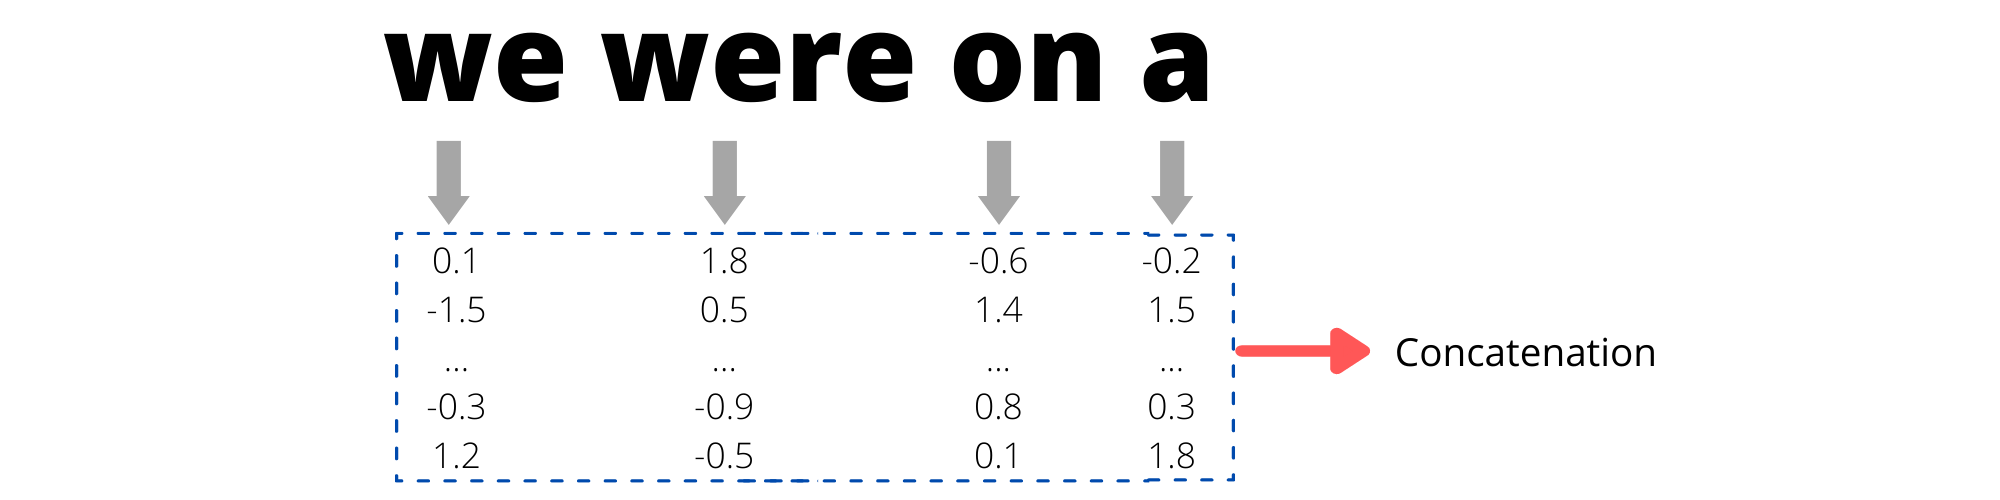
\includegraphics[width = 11cm]{images/NWP1.png}
\end{textblock}}
\only <2>{\begin{textblock}{0.15}(0.07, 0.6)
        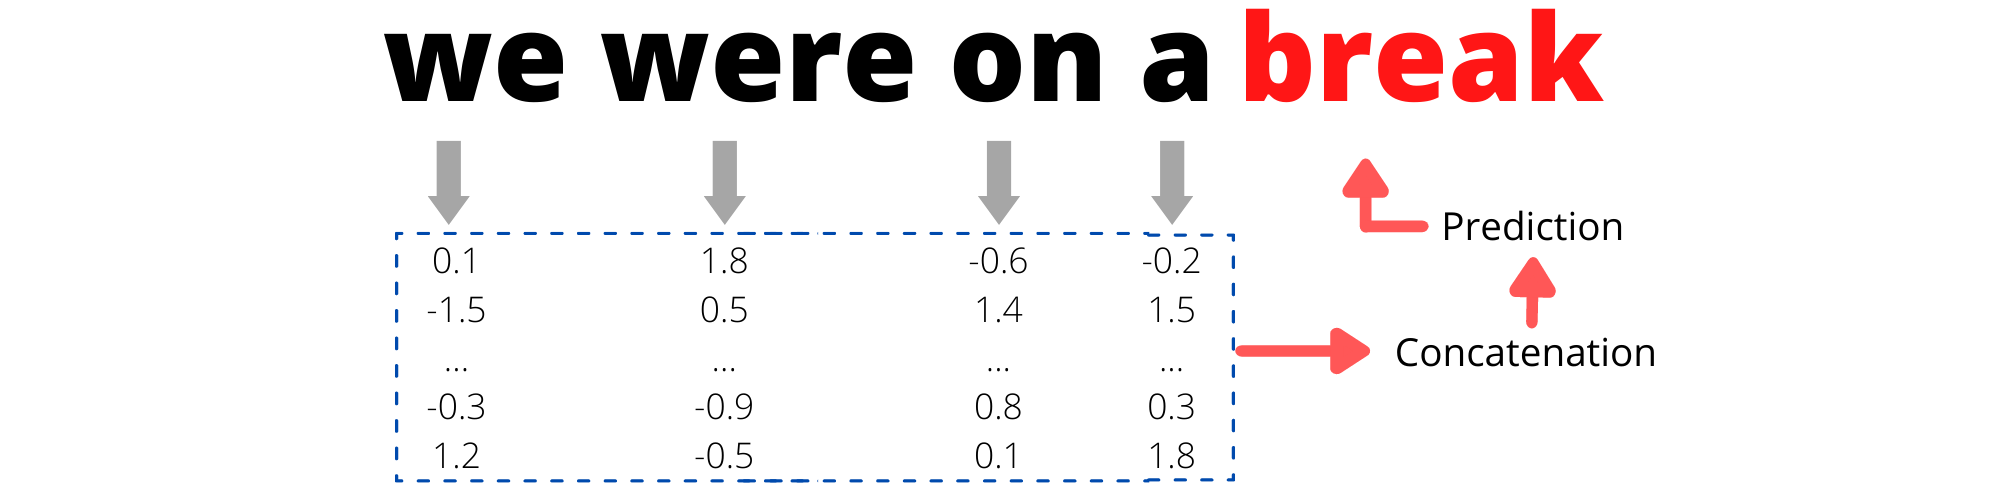
\includegraphics[width = 11cm]{images/NWP2.png}
\end{textblock}}
\only <3>{\begin{textblock}{0.15}(0.07, 0.6)
        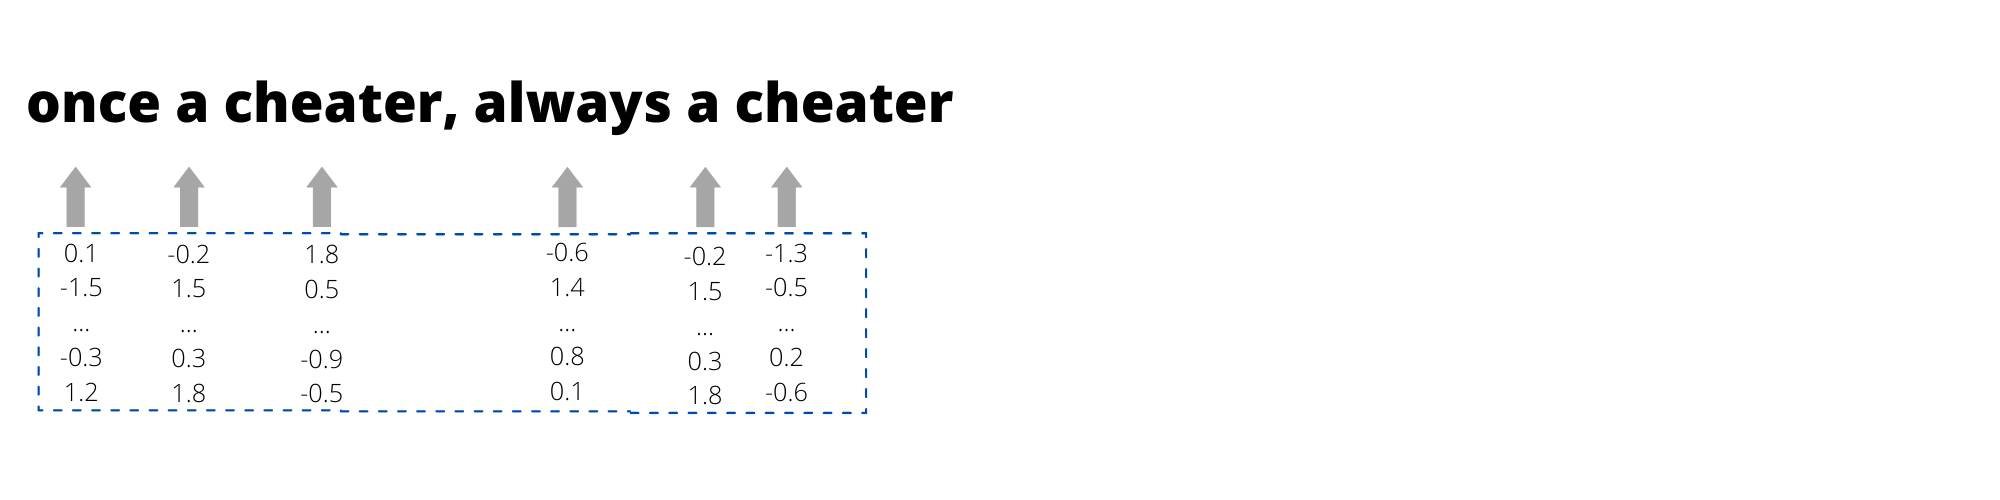
\includegraphics[width = 11cm]{images/NSP1.png}
\end{textblock}}
\only <4>{\begin{textblock}{0.15}(0.07, 0.6)
        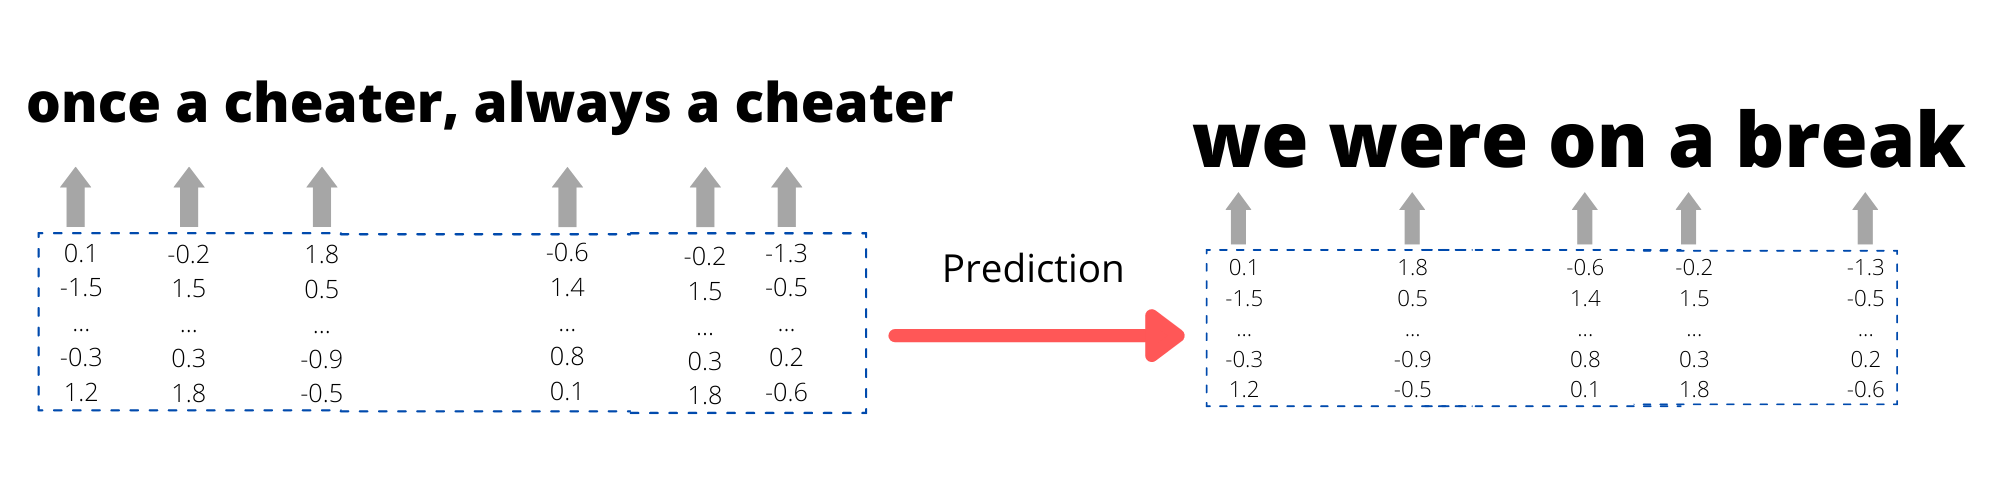
\includegraphics[width = 11cm]{images/NSP2.png}
\end{textblock}}
\only <5>{\begin{textblock}{0.15}(0.03, 0.6)
        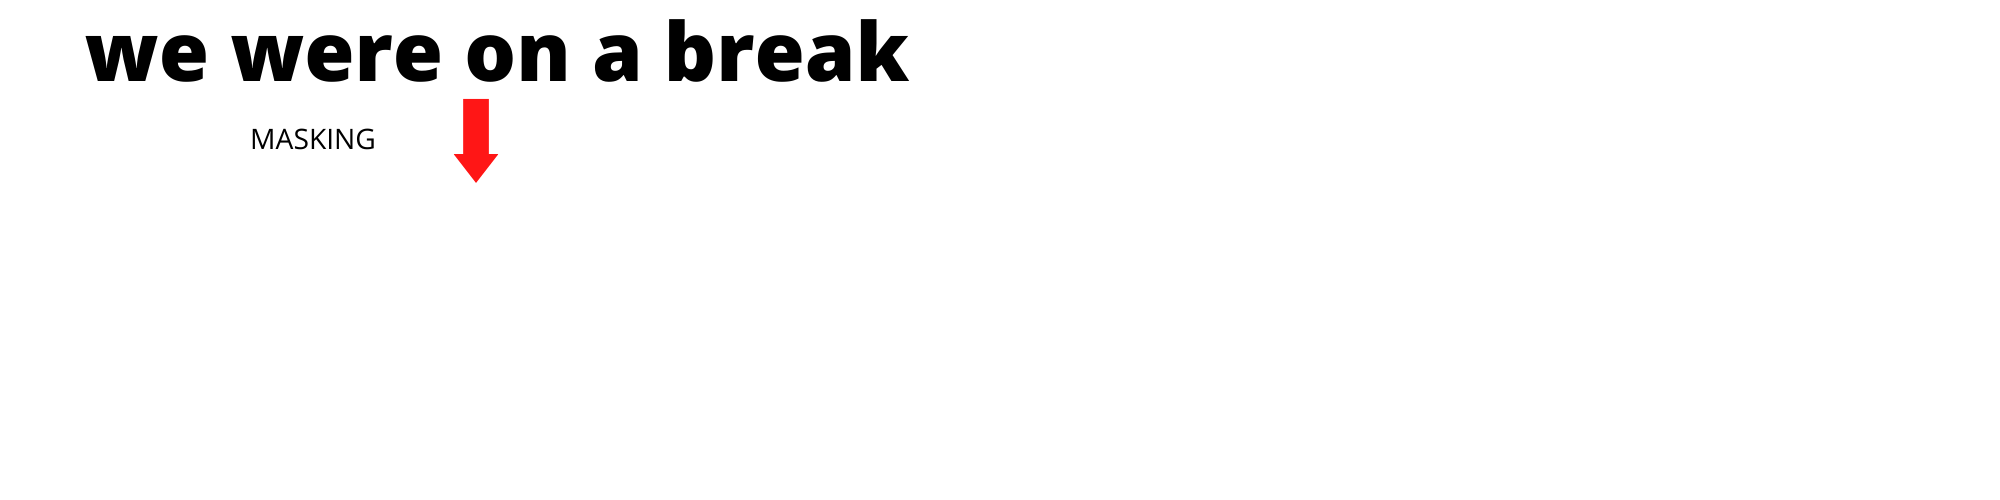
\includegraphics[width = 12cm]{images/MLM.png}
\end{textblock}}
\only <6>{\begin{textblock}{0.15}(0.03, 0.6)
        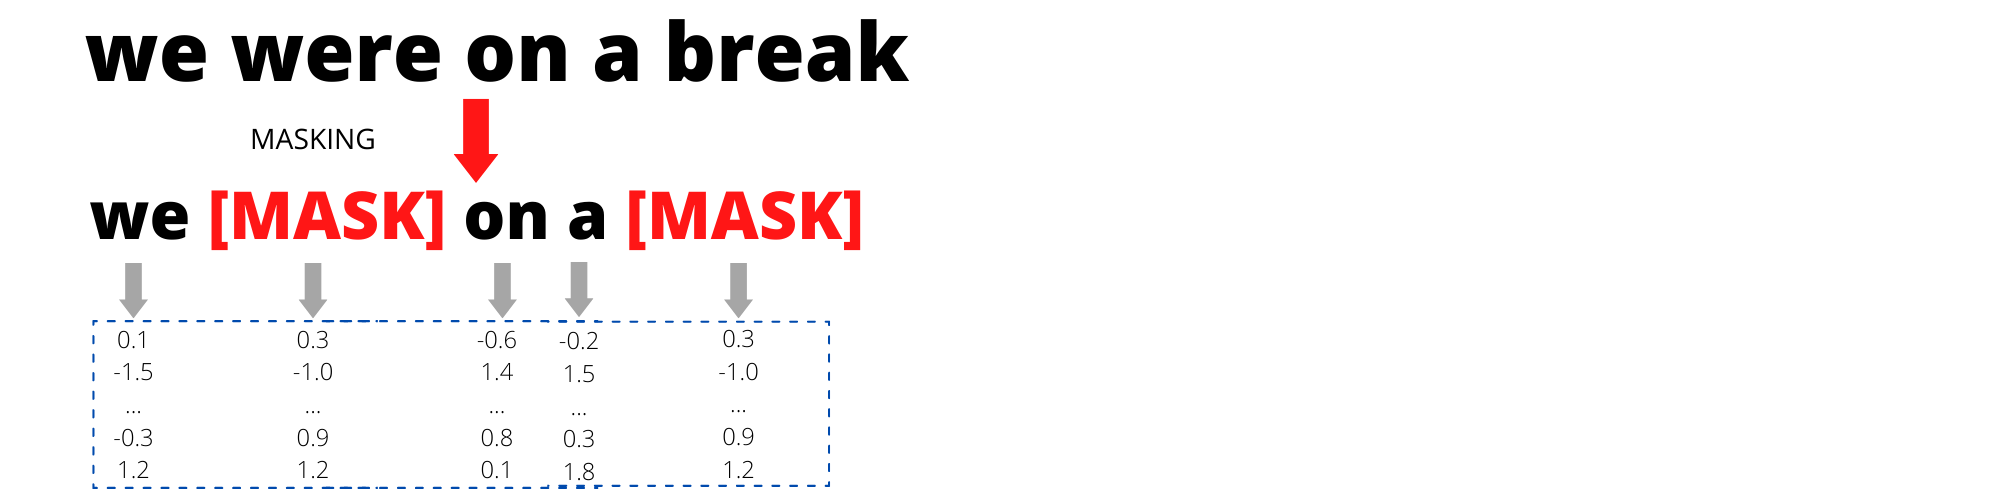
\includegraphics[width = 12cm]{images/MLM2.png}
\end{textblock}}
\only <7>{\begin{textblock}{0.15}(0.03, 0.6)
        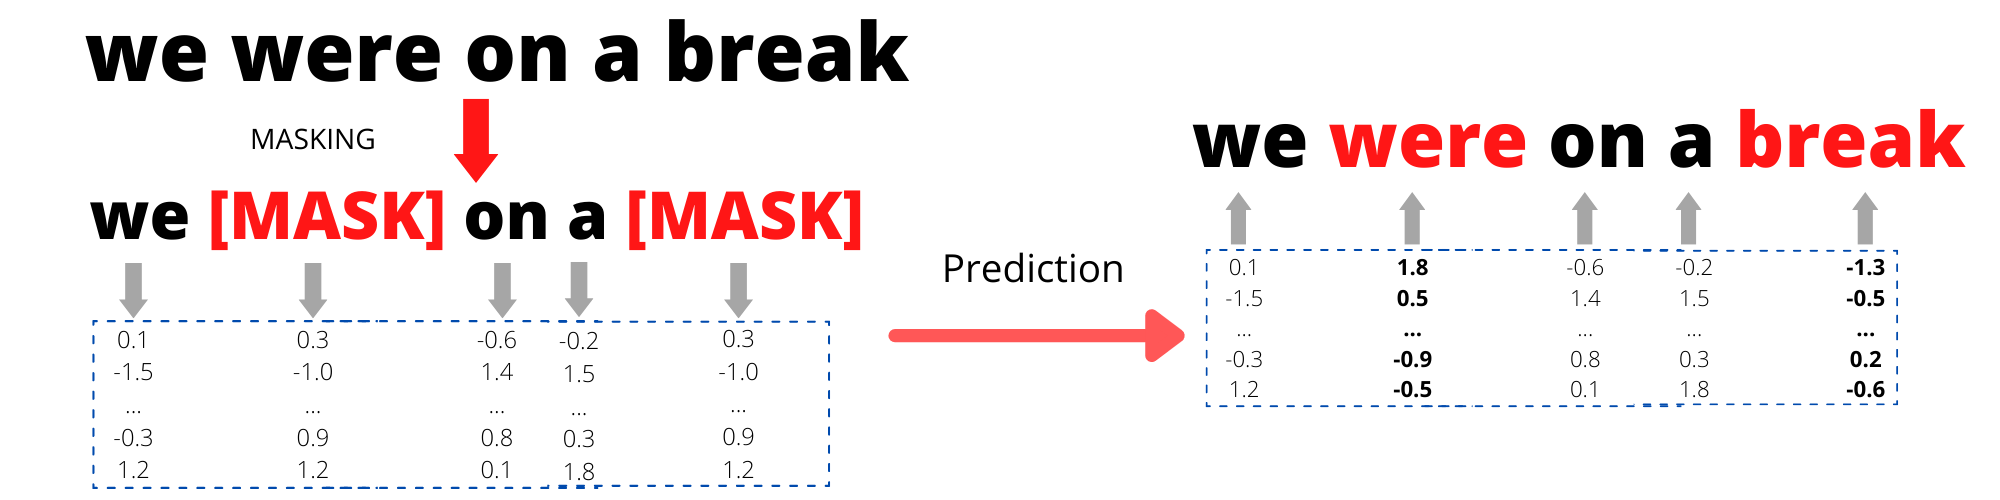
\includegraphics[width = 12cm]{images/MLM3.png}
\end{textblock}}
\end{frame}
\begin{frame}{Architectures for Language Modelling}
\vspace{0.3cm}\\
\begin{columns}[onlytextwidth]
    \begin{column}{0.50\textwidth}
    In Neural LM we combine vectors using \textbf{neural networks}. The simplest option is using a simple \textbf{Multi-layer perceptron} as in Bengio et al. \cite{bengio}. %explain further
    However, this is arguably not the best option to encode language.
    \vspace{0.2cm}\\ We will go through two more options that are widely used today:
    \begin{itemize}
        \item Recurrent Neural Networks (RNN)
        \item Transformers
    \end{itemize}
    \end{column}
\end{columns}
\begin{textblock}{0.5}(0.50, 0.25)
        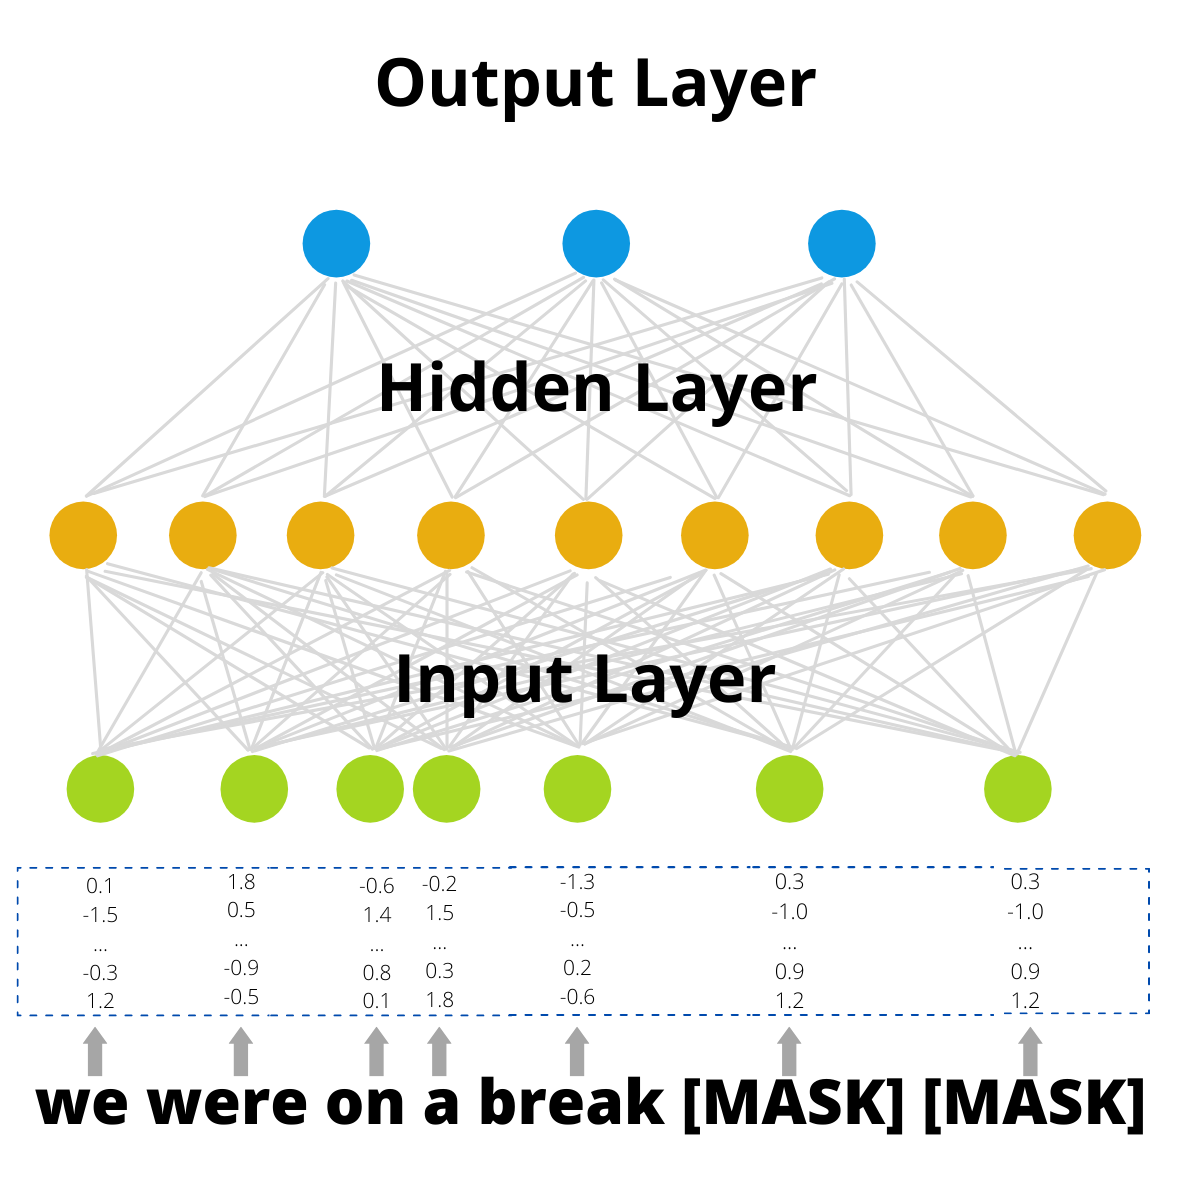
\includegraphics[width = 6cm]{images/MLP.png}
\end{textblock}
\end{frame}

\section{Recurrent Neural Networks}
\begin{frame}
    \frametitle{Table of contents}
    \tableofcontents[currentsection]
\end{frame}
\subsection{Vanilla RNN}
\begin{frame}{Recurrent Neural Networks}
%\vspace{0.3cm}\\
    RNNs are an ideal solution to deal with sequences of unknown length. In its simple version (\textbf{Vanilla RNN}) we simply apply a neural network to generate an \textbf{output} and a \tetxbf{hidden state} to every member of the sequence.
\only <1>{
\begin{textblock}{0.15}(0.07, 0.39)
        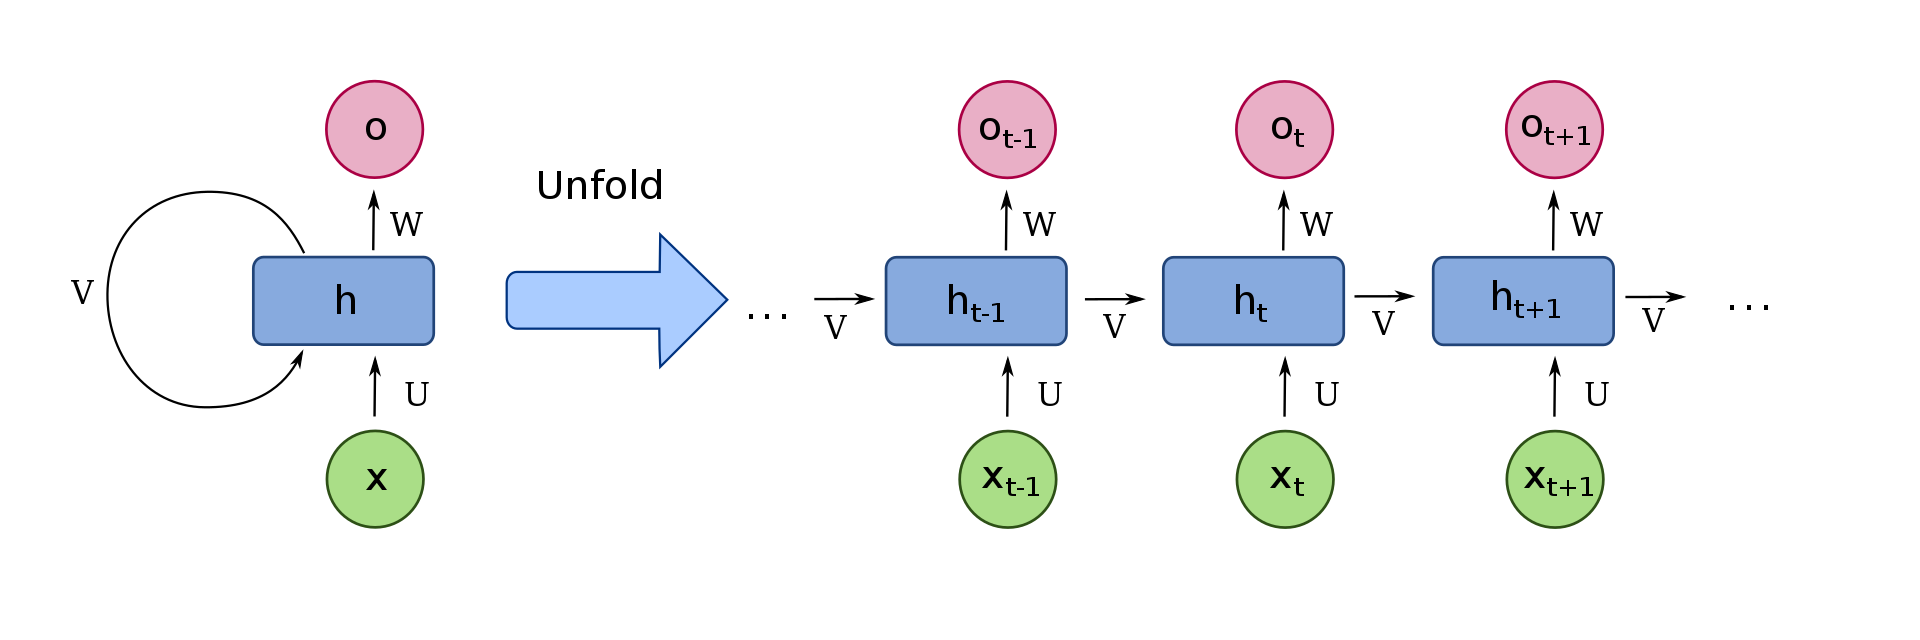
\includegraphics[width = 11cm]{images/rnn.png}
\end{textblock}}
\only <2>{
\begin{textblock}{0.15}(0.07, 0.39)
        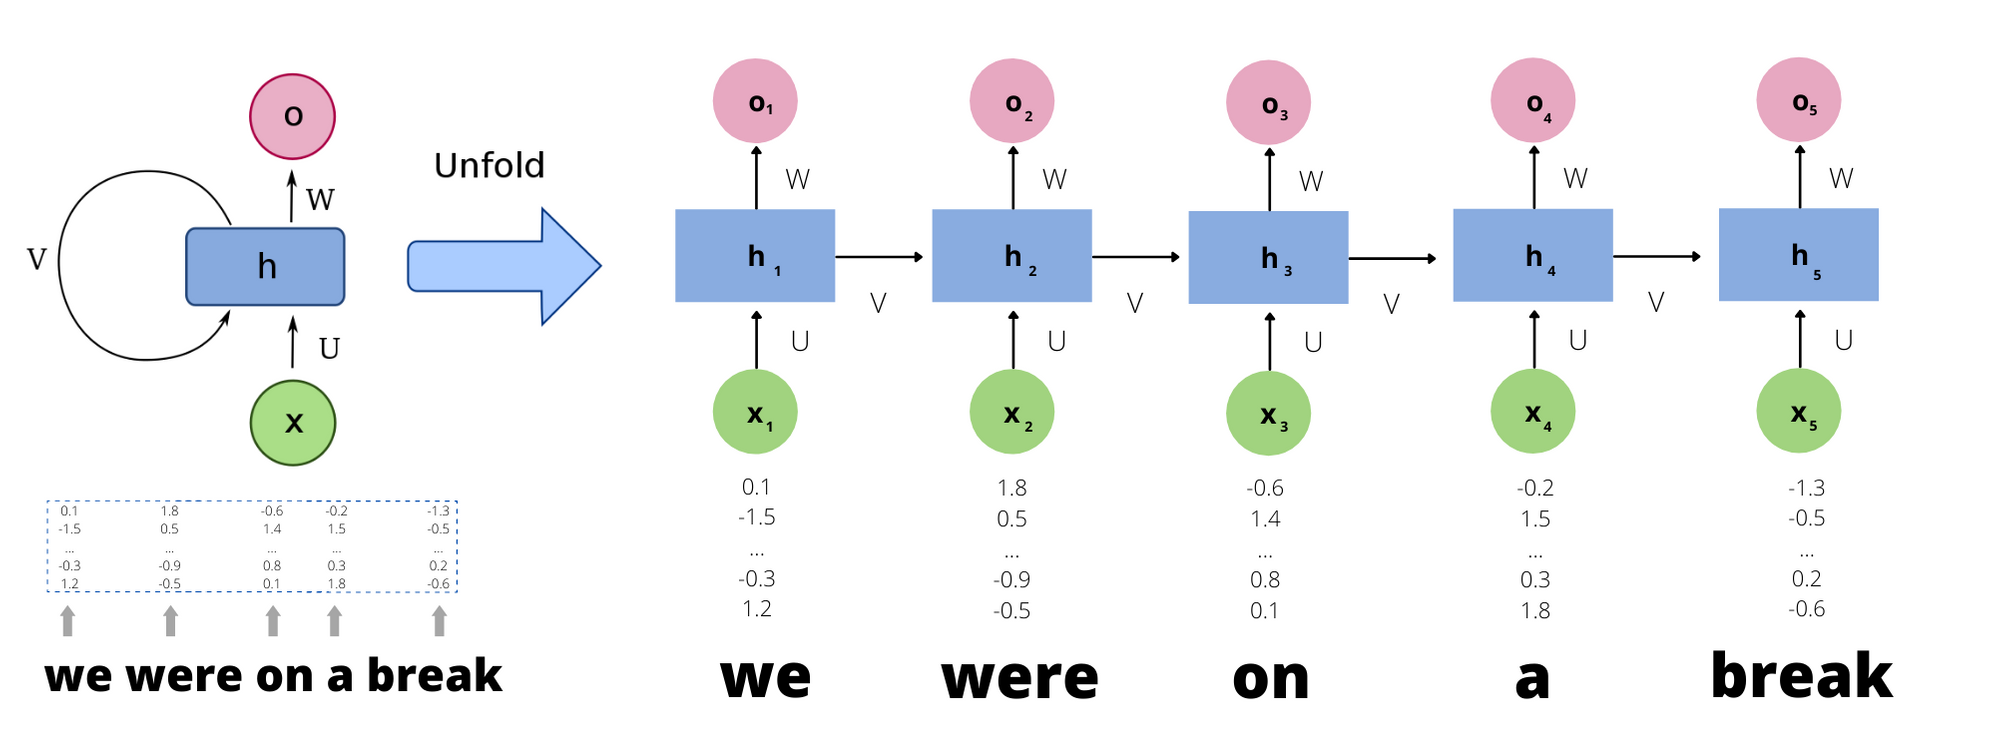
\includegraphics[width = 11cm]{images/rnn_example.png}
\end{textblock}}
    \vspace{4.5cm}\\ For any given word, we apply both the input vector and the previous hidden state.
\end{frame}
\subsection{RNNs in Practice}
\begin{frame}{Bi-directional LSTM}
\vspace{0.3cm}\\
    RNNs are not perfect: in particular, they suffer from the \textbf{vanishing gradient problem}. This is, when we back-propagate the error to update the weights, we loose information, particularly with long sequences.\\
    In reality, we often apply \textbf{bi-directionality}\only <2> { and we use a more complex architecture instead: the \textbf{Long Short Term Memory Network}}.
\only <1>{
\begin{textblock}{0.15}(0.07, 0.45)
        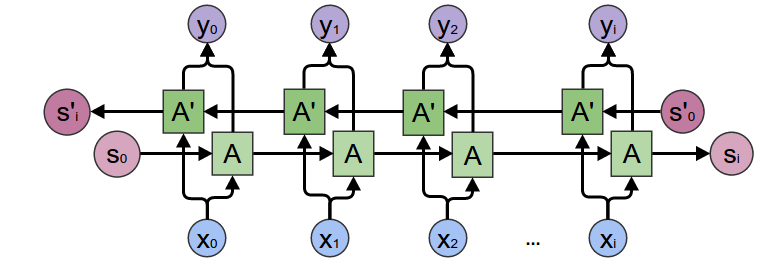
\includegraphics[width = 11cm]{images/bidirectional.png}
\end{textblock}}
\only <2>{
\begin{textblock}{0.15}(0.07, 0.49)
        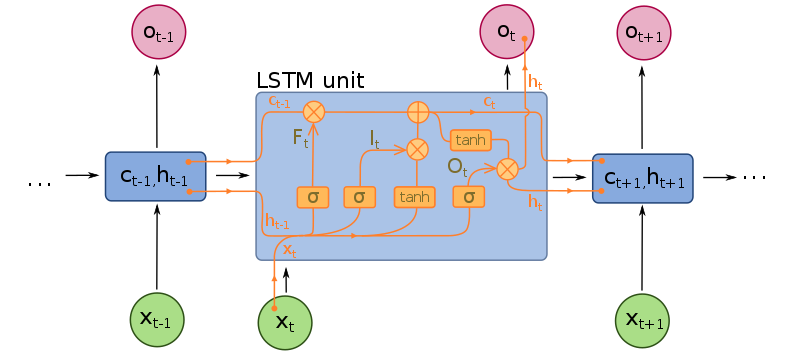
\includegraphics[width = 10cm]{images/lstm.png}
\end{textblock}}
\end{frame}

\section{Attention}
\begin{frame}
    \frametitle{Table of contents}
    \tableofcontents[currentsection]
\end{frame}
\begin{frame}{RNNs: a Machine Translation example}
    Let's consider an example of \textbf{machine translation}. We will consider an RNN for \textbf{encoding} the input sequence and another one for \textbf{decoding} it into the output sequence.
    \only <1>{
\begin{textblock}{0.15}(0.03, 0.4)
        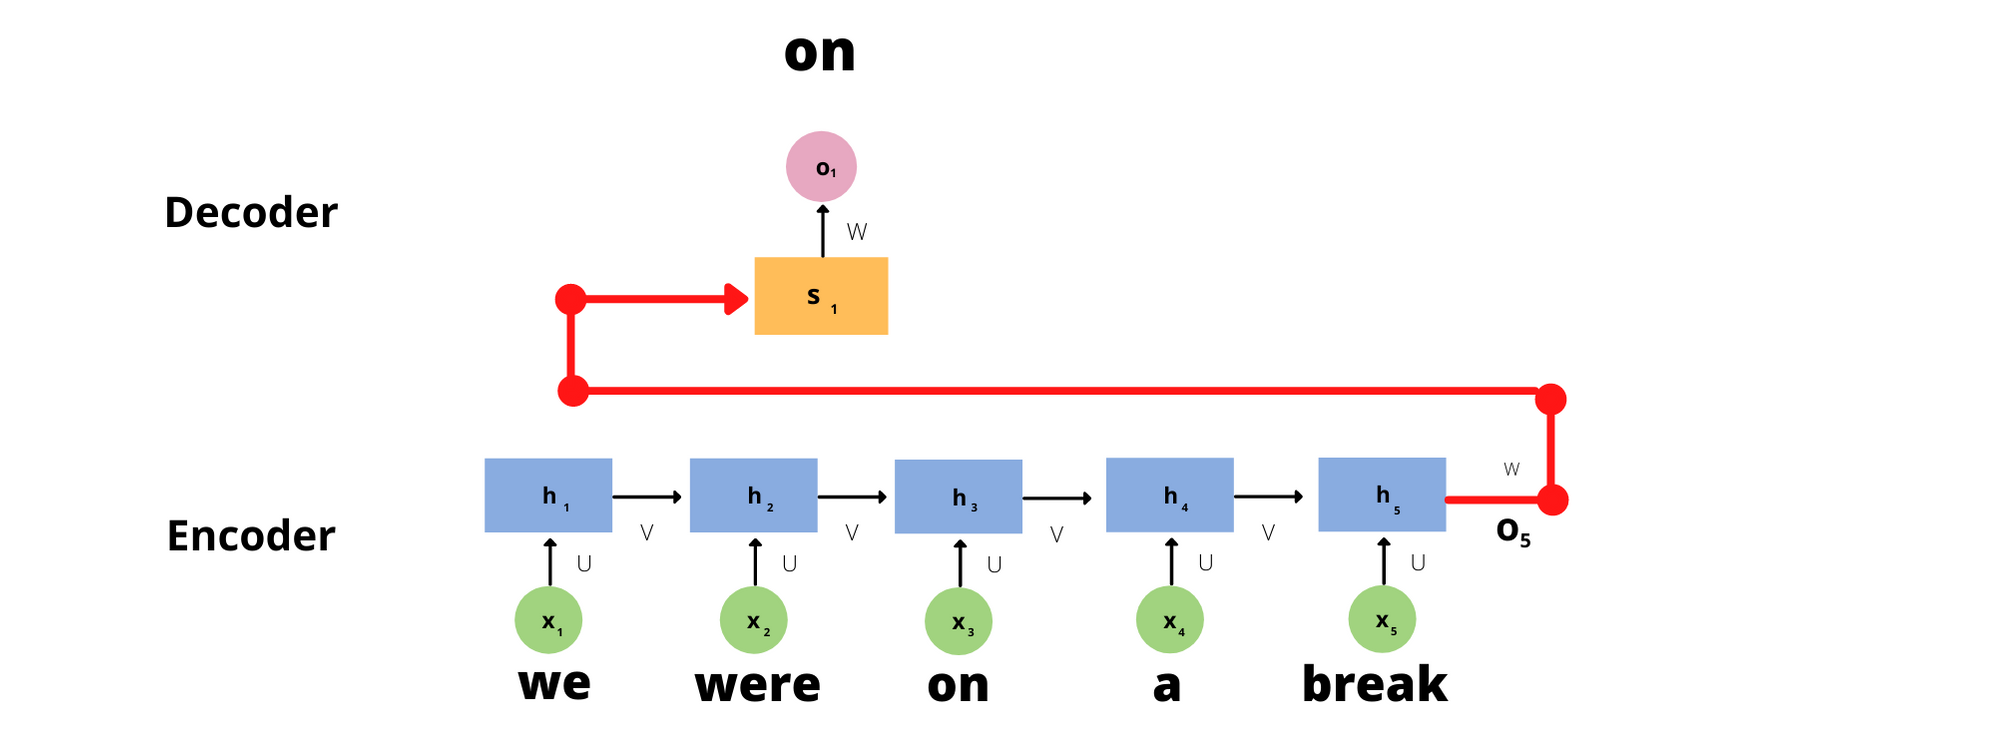
\includegraphics[width = 13cm]{images/RNN_ML1.png}
\end{textblock}}
    \only <2>{
\begin{textblock}{0.15}(0.03, 0.4)
        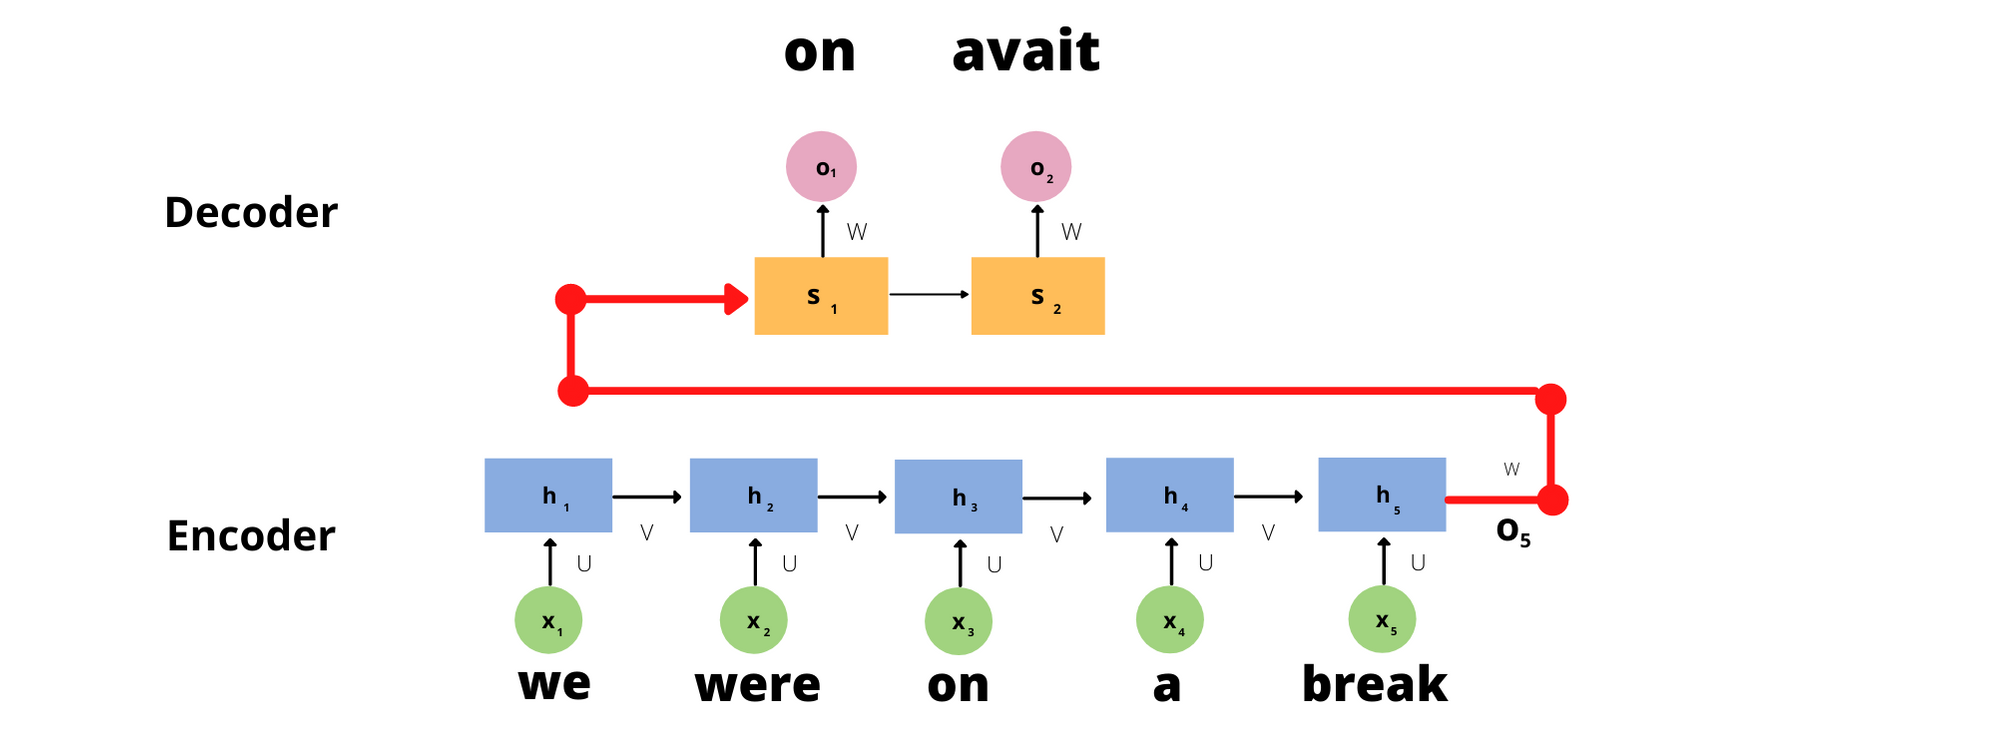
\includegraphics[width = 13cm]{images/RNN_ML2.png}
\end{textblock}}
    \only <3>{
\begin{textblock}{0.15}(0.03, 0.4)
        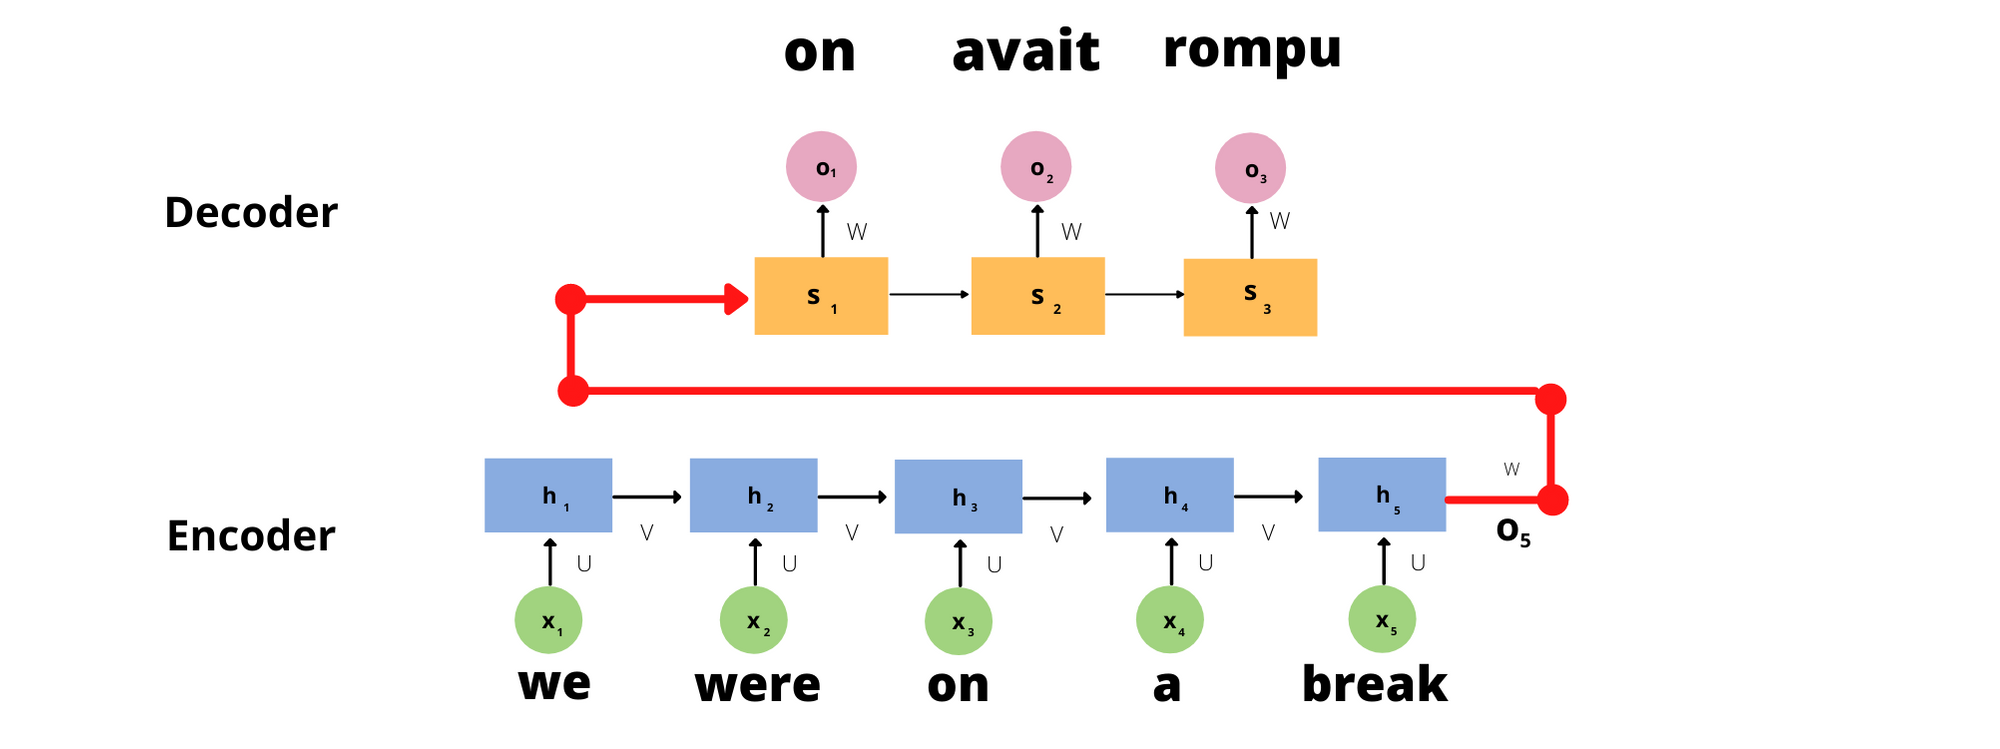
\includegraphics[width = 13cm]{images/RNN_ML3.png}
\end{textblock}}
\end{frame}
\begin{frame}{RNNs: a Machine Translation example}
    A drawback of such a setting is that by encoding the whole sentence in the last output, we are not pushing the decoder to \textbf{focus on the important parts of the input}.
    For example, for computing \textbf{on} in French, we only need to pay attention to the word \textbf{we} in English. 
\begin{textblock}{0.15}(0.03, 0.4)
        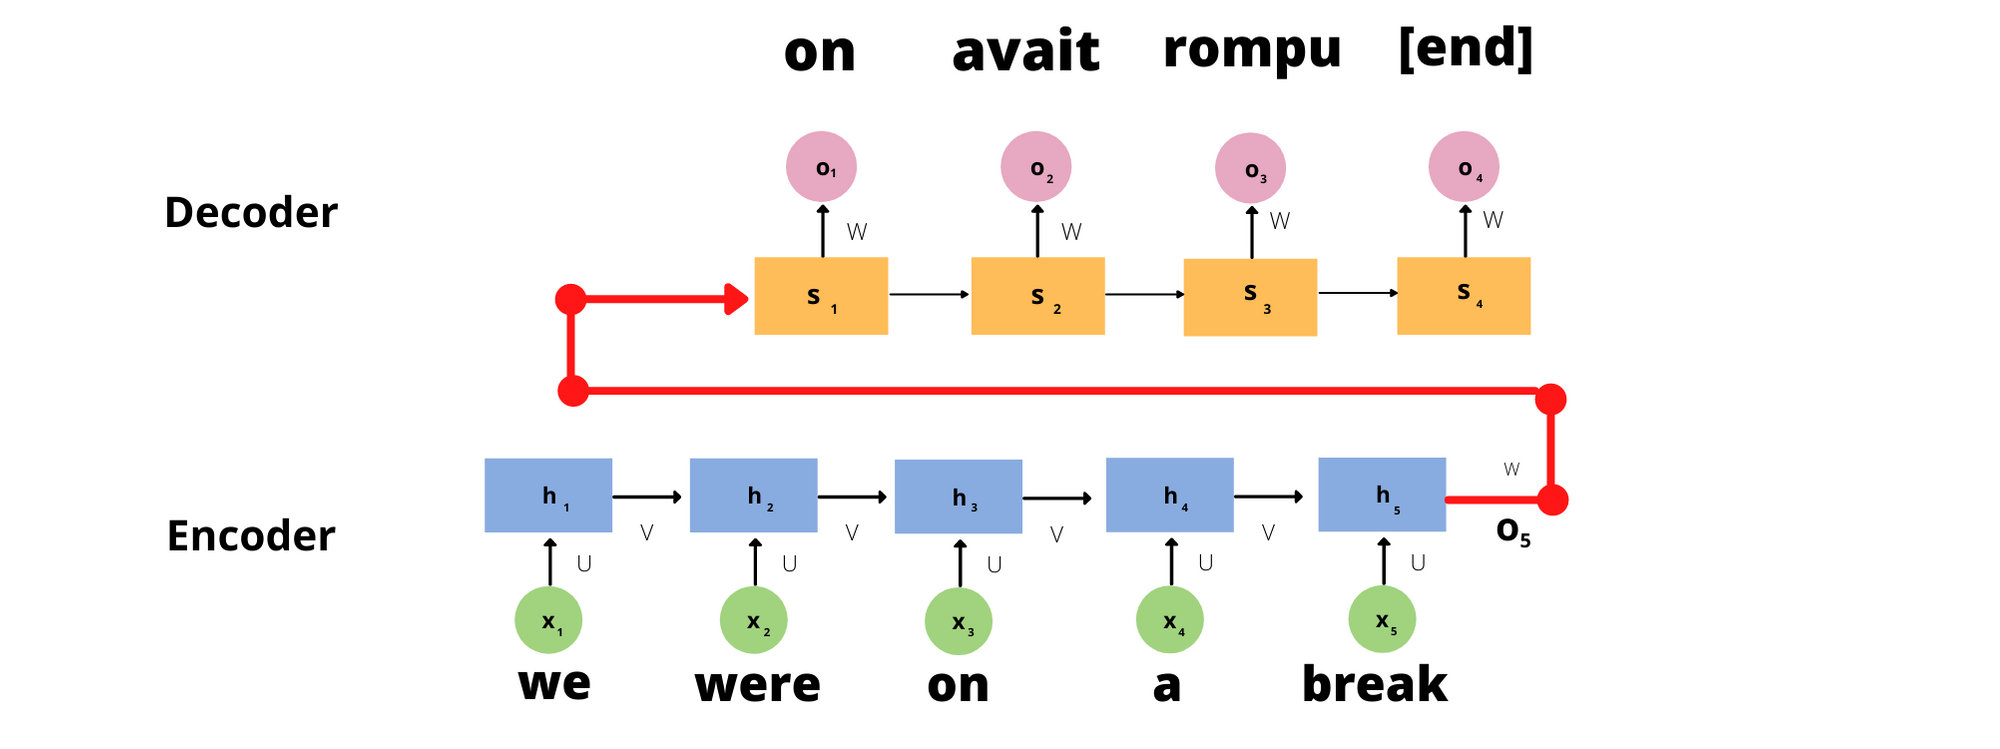
\includegraphics[width = 13cm]{images/RNN_ML4.png}
\end{textblock}
\end{frame}
\iffalse %%%%% IGNORING FRAME
\begin{frame}{Attention Modules}
    Let $x=x_1,\dots,x_n$ and $y_1,\dots,y_m$ be the input and output sequences respectively. Let $h=h_1,\dots,h_n$ and $s=s_1,\dots,s_m$ be the respective hidden states, with the encoder being a bi-directional RNN and the decoder given by $s_t=f(s_{t-1},y_{t-1},c_t)$ with $c_t$ a context vector. These context vectors will be the sum of the hidden states from the input sequence, weighted by an \textbf{alignment score}.
    $$ c_t = \displaystyle \sum^n_{i=1}\alpha_{t,i}h_i $$
    $$ \alpha_{t,i} = softmax(score(s_{t-1},h_i))  $$
    Originally, the score corresponds to a feed forward neural network: $score(s_t,h_i) = v_a^Ttanh(W_a[s_t,h_i])$ with learnable $v_a$ and $W_a$ 
\end{frame} \fi
\begin{frame}{Attention}
Attention tries to overcome the challenge we mentioned on the previous slide by making \textbf{direct connections} between output tokens and the \textbf{important tokens} on the input that correspond to it. \only <1,2> {Let's look at our example again:}
\only <3> {Moreover, we want the module to \textbf{attend more} to \textbf{more important tokens}.}
\only <1> {
\begin{textblock}{0.15}(0.03, 0.4)
        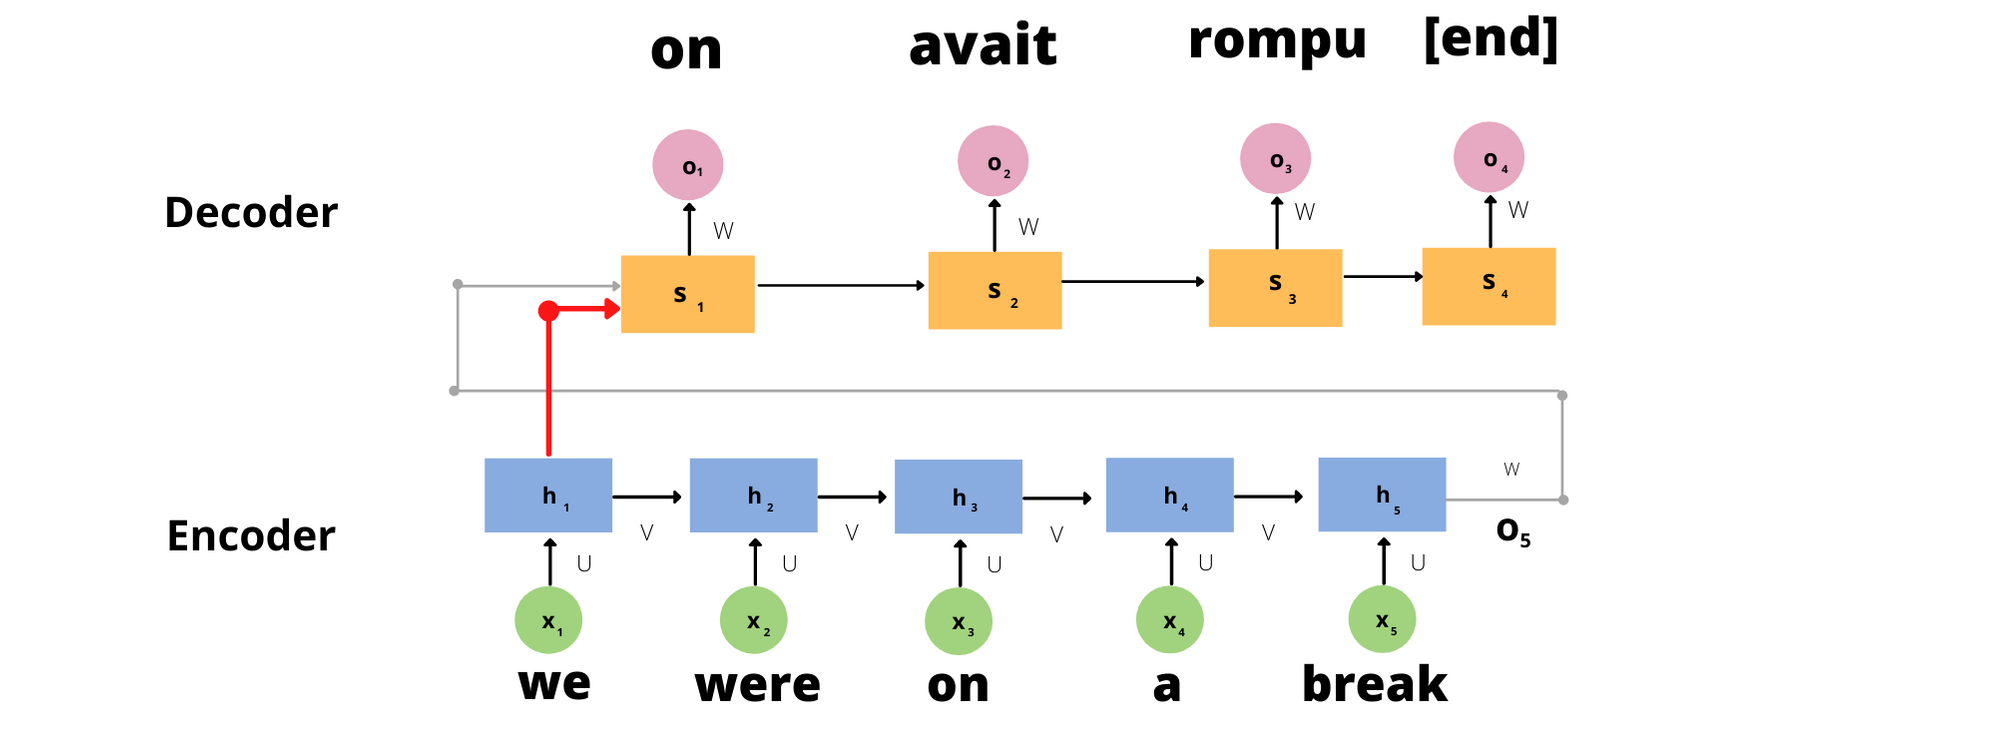
\includegraphics[width = 13cm]{images/attn_intuiton1.png}
\end{textblock}}
\only <2> {
\begin{textblock}{0.15}(0.03, 0.4)
        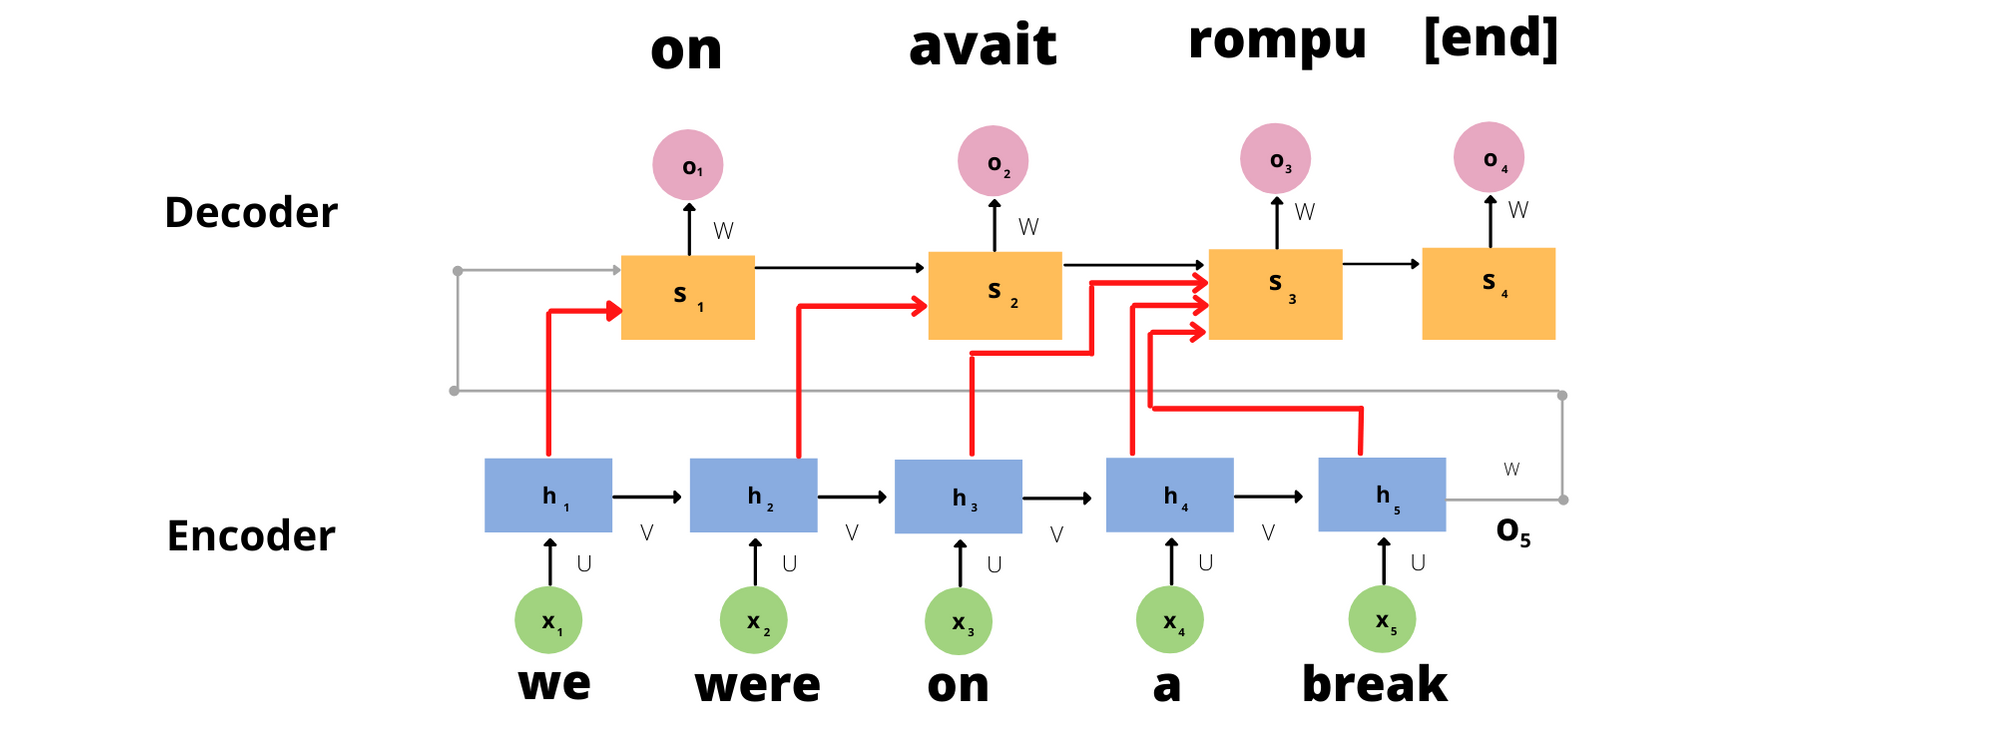
\includegraphics[width = 13cm]{images/attn_intuiton2.png}
\end{textblock}}
\only <3> {
\begin{textblock}{0.15}(0.03, 0.45)
        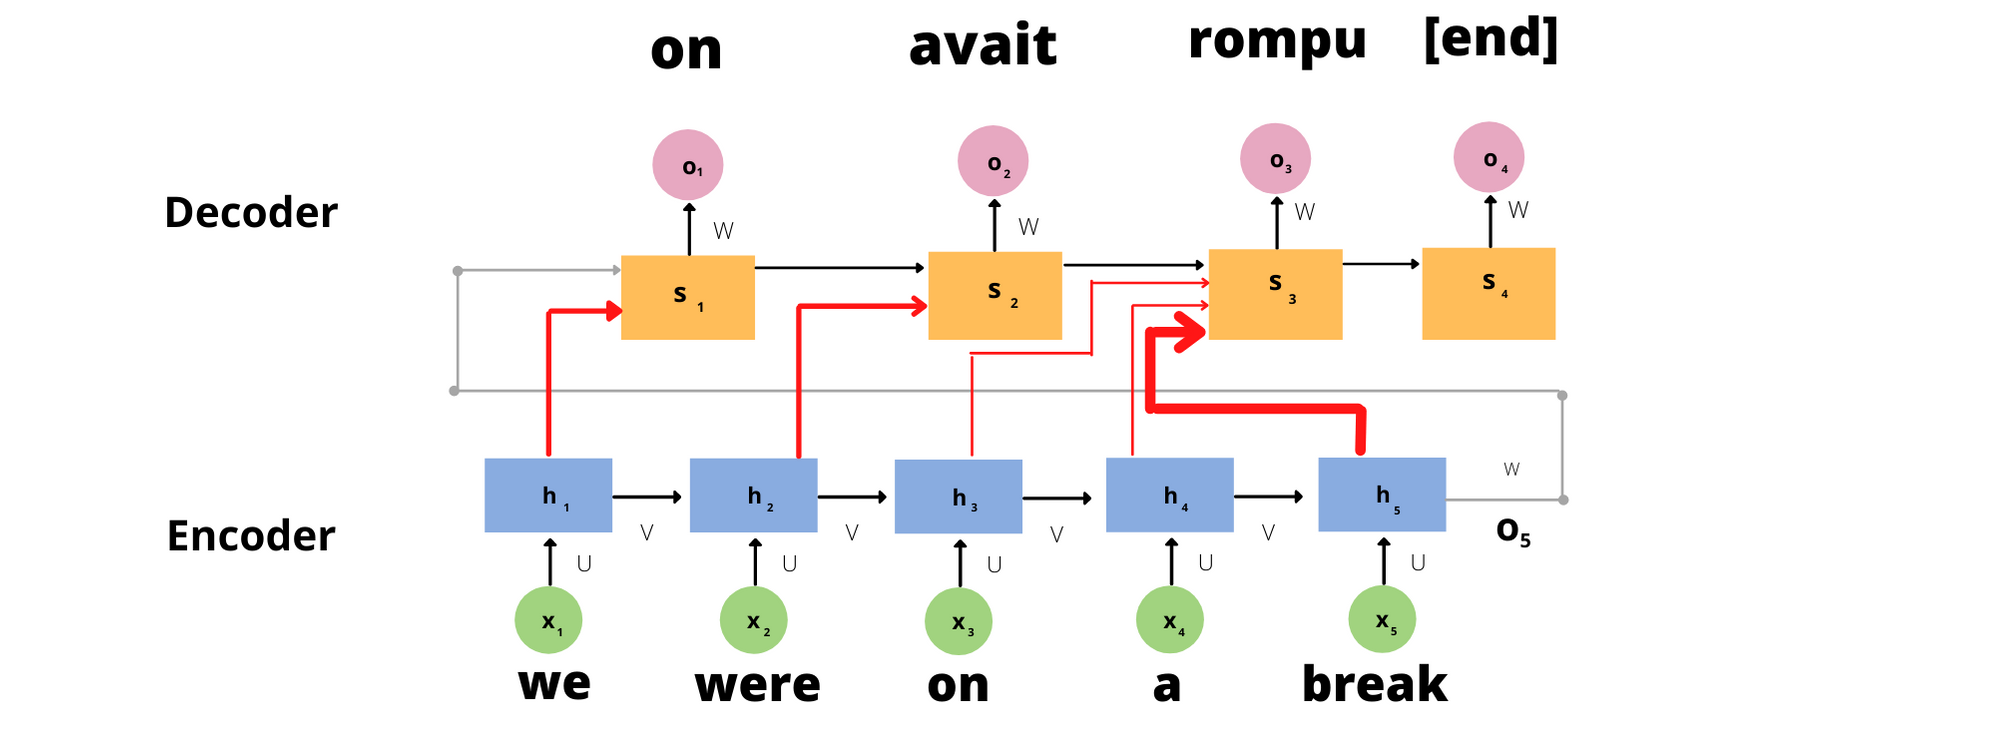
\includegraphics[width = 13cm]{images/attn_intuiton3.png}
\end{textblock}}
\end{frame}
\begin{frame}{Attention Modules} %%%%
\vspace{0.3cm}\\
    In other words, attention allows a direct interaction between different token positions by introducing a \tetxbf{weighted average} of the previous RNN layers into the next one.
\only <1> {
\begin{textblock}{0.15}(0.03, 0.4)
        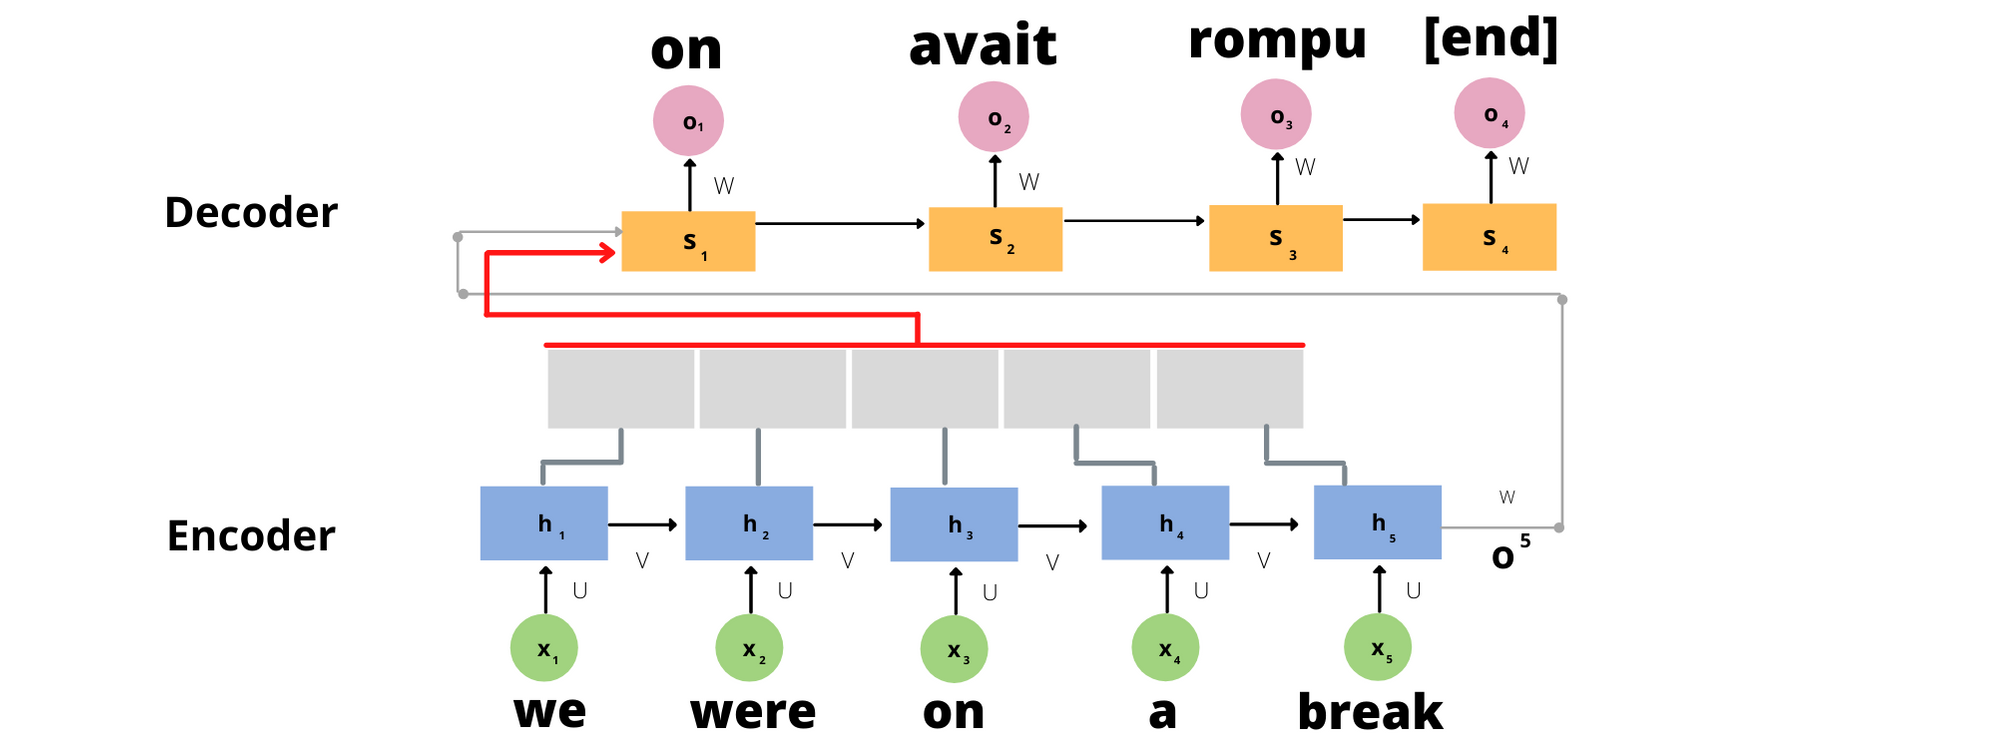
\includegraphics[width = 13cm]{images/attn_layer1.png}
\end{textblock}}
\only <2> {
\begin{textblock}{0.15}(0.03, 0.4)
        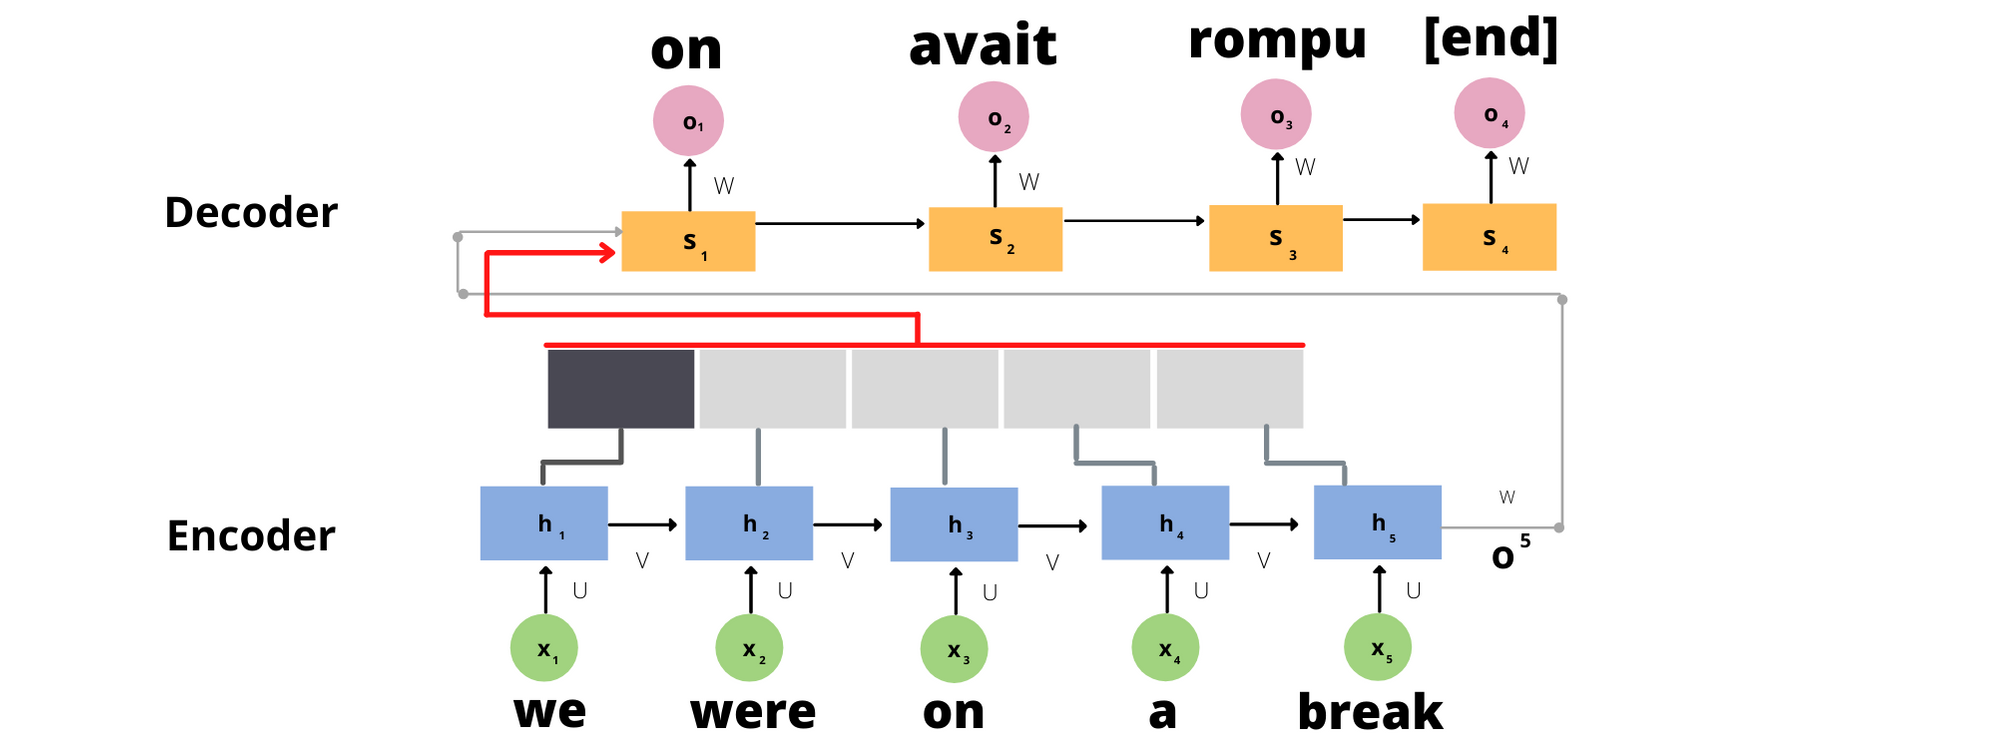
\includegraphics[width = 13cm]{images/attn_layer2.png}
\end{textblock}}
\only <3> {
\begin{textblock}{0.15}(0.03, 0.4)
        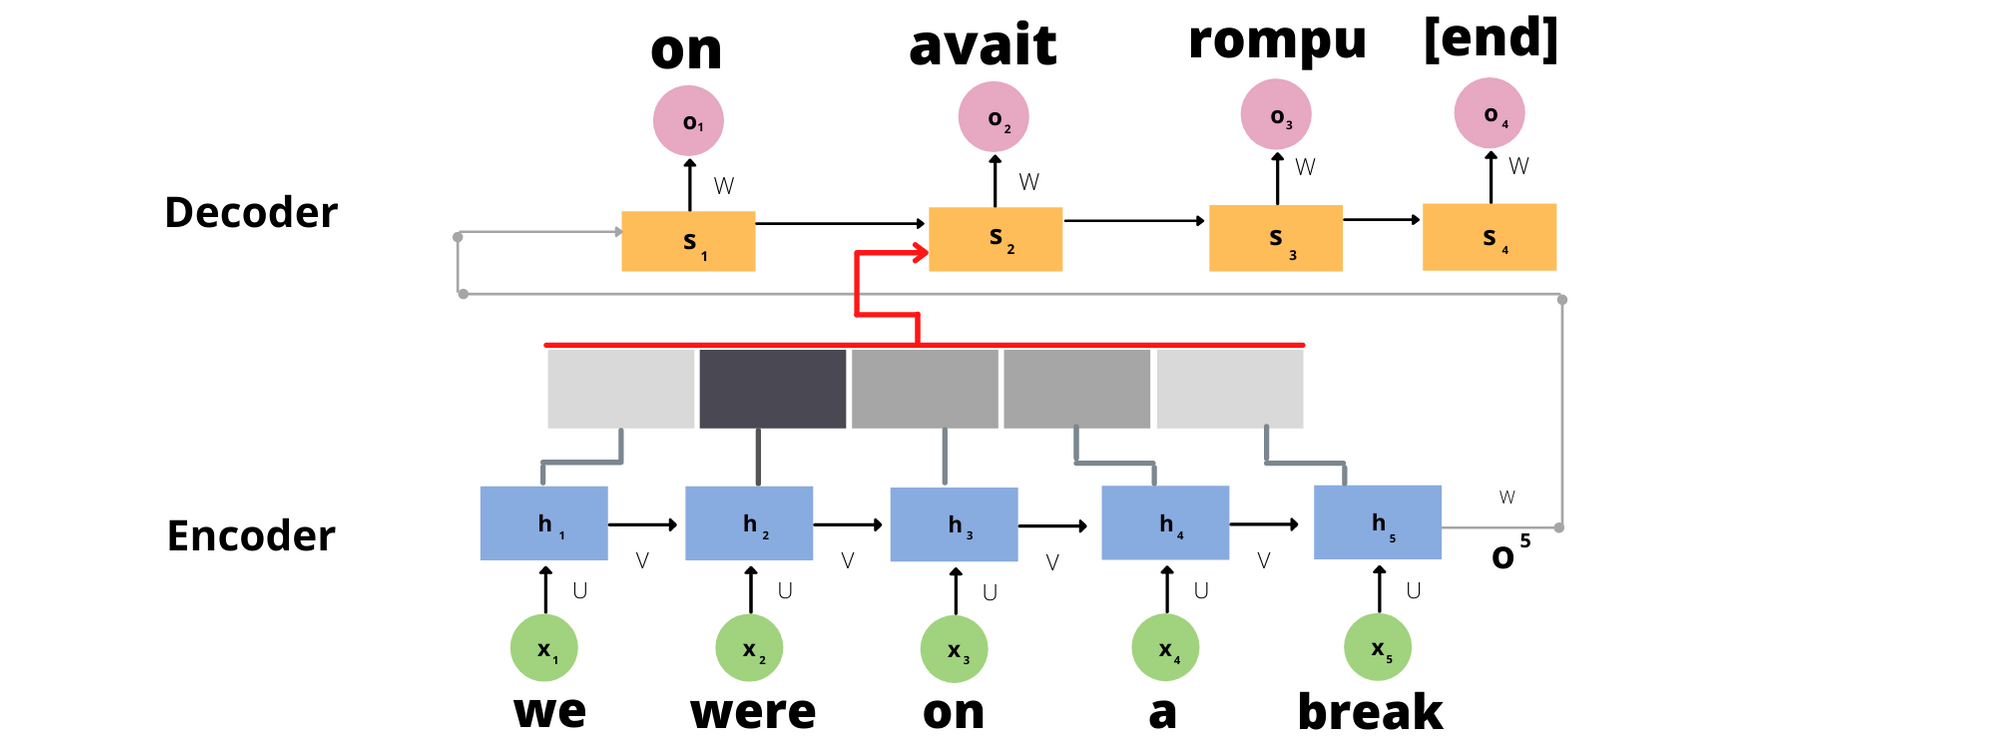
\includegraphics[width = 13cm]{images/attn_layer3.png}
\end{textblock}}
\only <4> {
\begin{textblock}{0.15}(0.03, 0.4)
        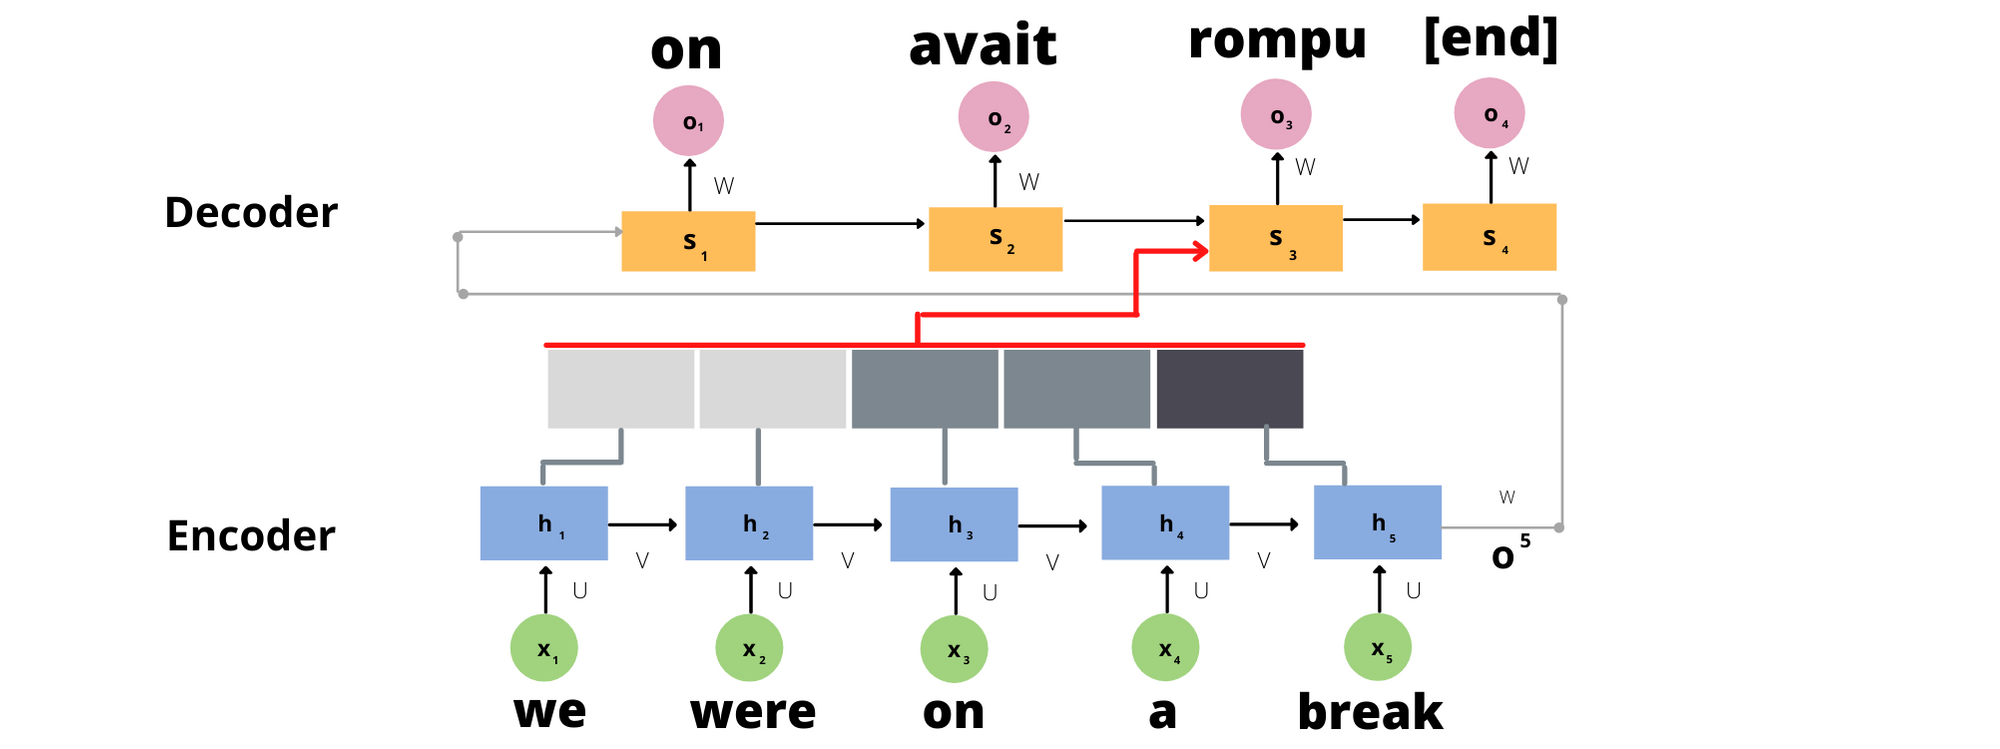
\includegraphics[width = 13cm]{images/attn_layer4.png}
\end{textblock}}
\end{frame}
\begin{frame}{Attention Modules}
\begin{columns}[onlytextwidth]
    \begin{column}{0.50\textwidth}
    We end up with a structure that resembles a \textbf{matrix}. The attention scores encode pairwise dependencies.\\
    \only <2,3,4,5,6> {More generally, we will refer to \textbf{queries (q)}, \textbf{values (v)} and \textbf{(keys (k))}. In this case we have:
    $$ A(q,K,V) = softmax(score(q,K))V$$
    $$score(s_t,h_i) = v_a^Ttanh(W_a[s_t,h_i])$$
    with learnable $v_a$ and $W_a$. Both $k,v=h_i$ come from the input RNN, while $q=s_t$ comes from the output. }
    \end{column}
\end{columns}
\only <1>{
\begin{textblock}{0.5}(0.55, 0.15)
        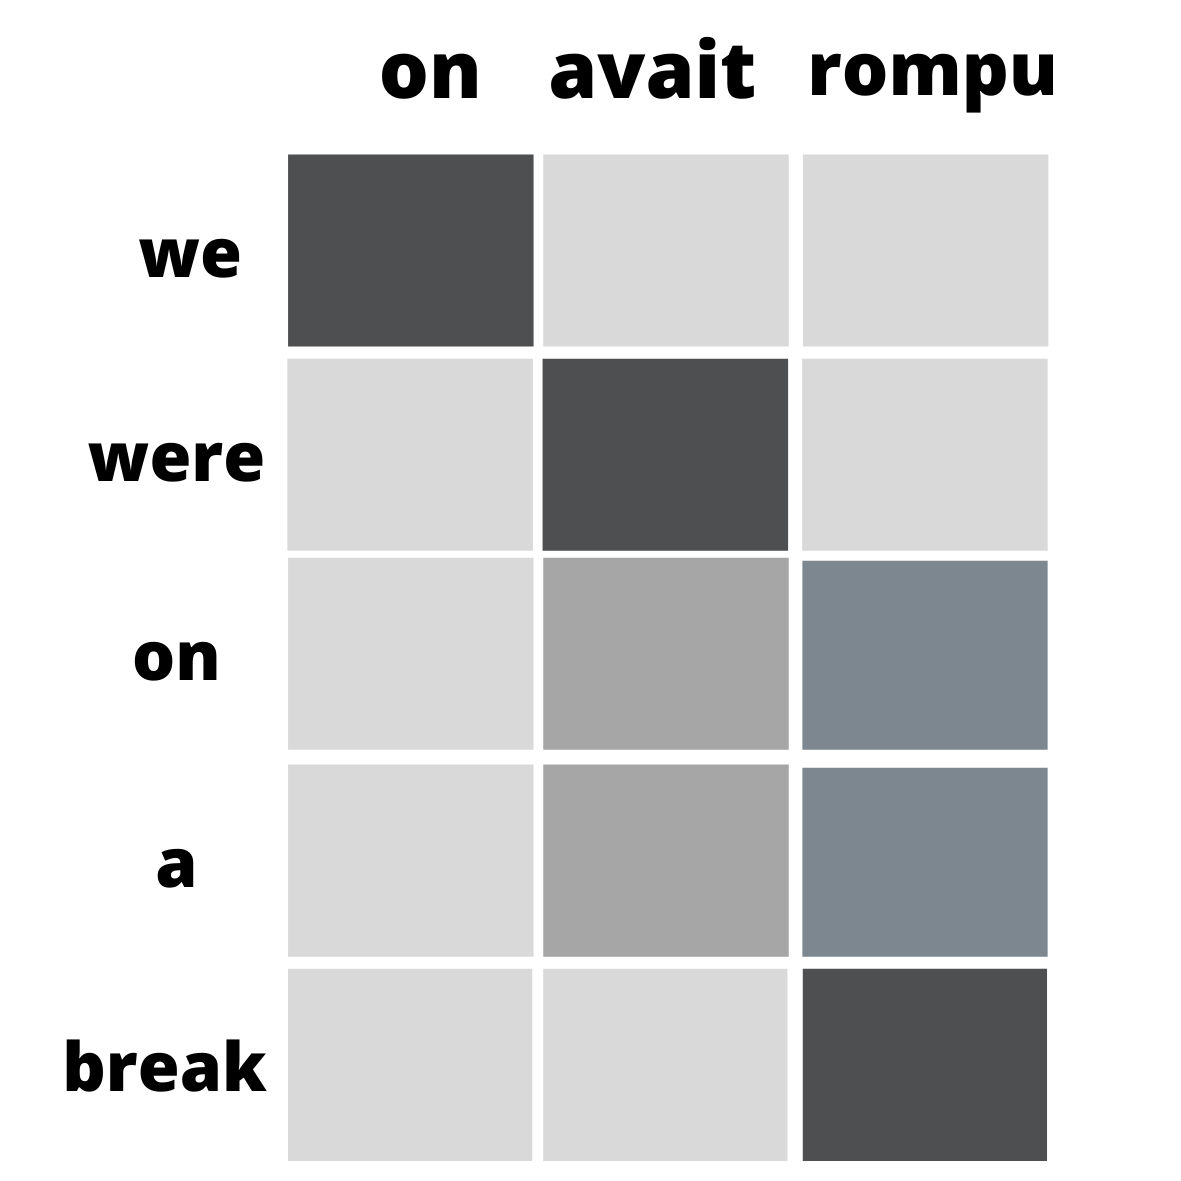
\includegraphics[width = 6cm]{images/attn_matrix.png}
\end{textblock}}
\only <2>{
\begin{textblock}{0.5}(0.55, 0.15)
        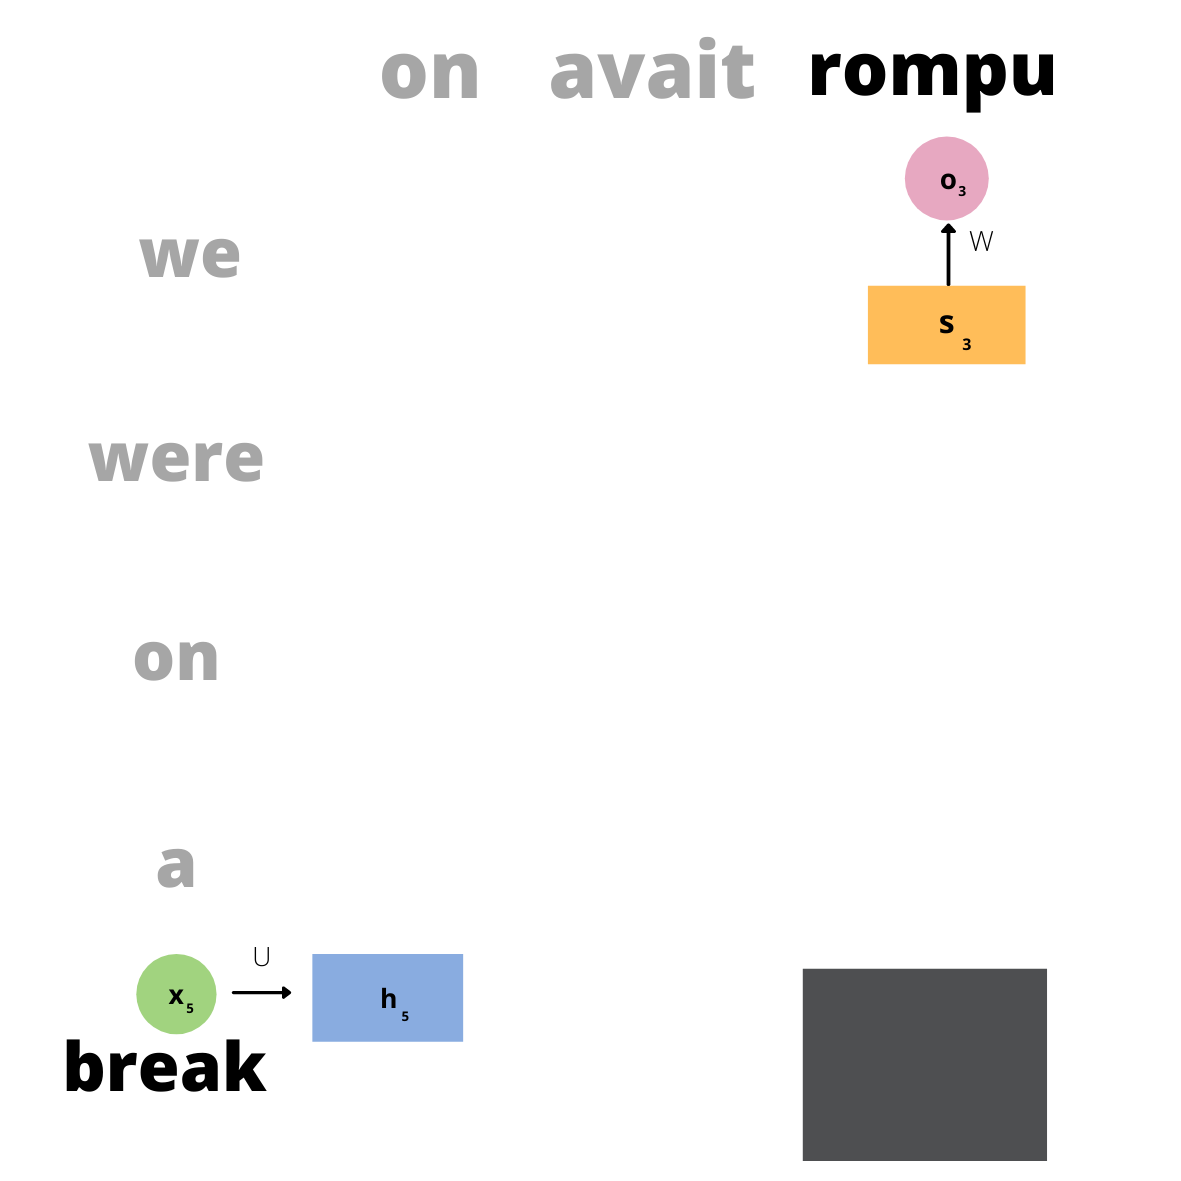
\includegraphics[width = 6cm]{images/attn_structure1.png}
\end{textblock}}
\only <3>{
\begin{textblock}{0.5}(0.55, 0.15)
        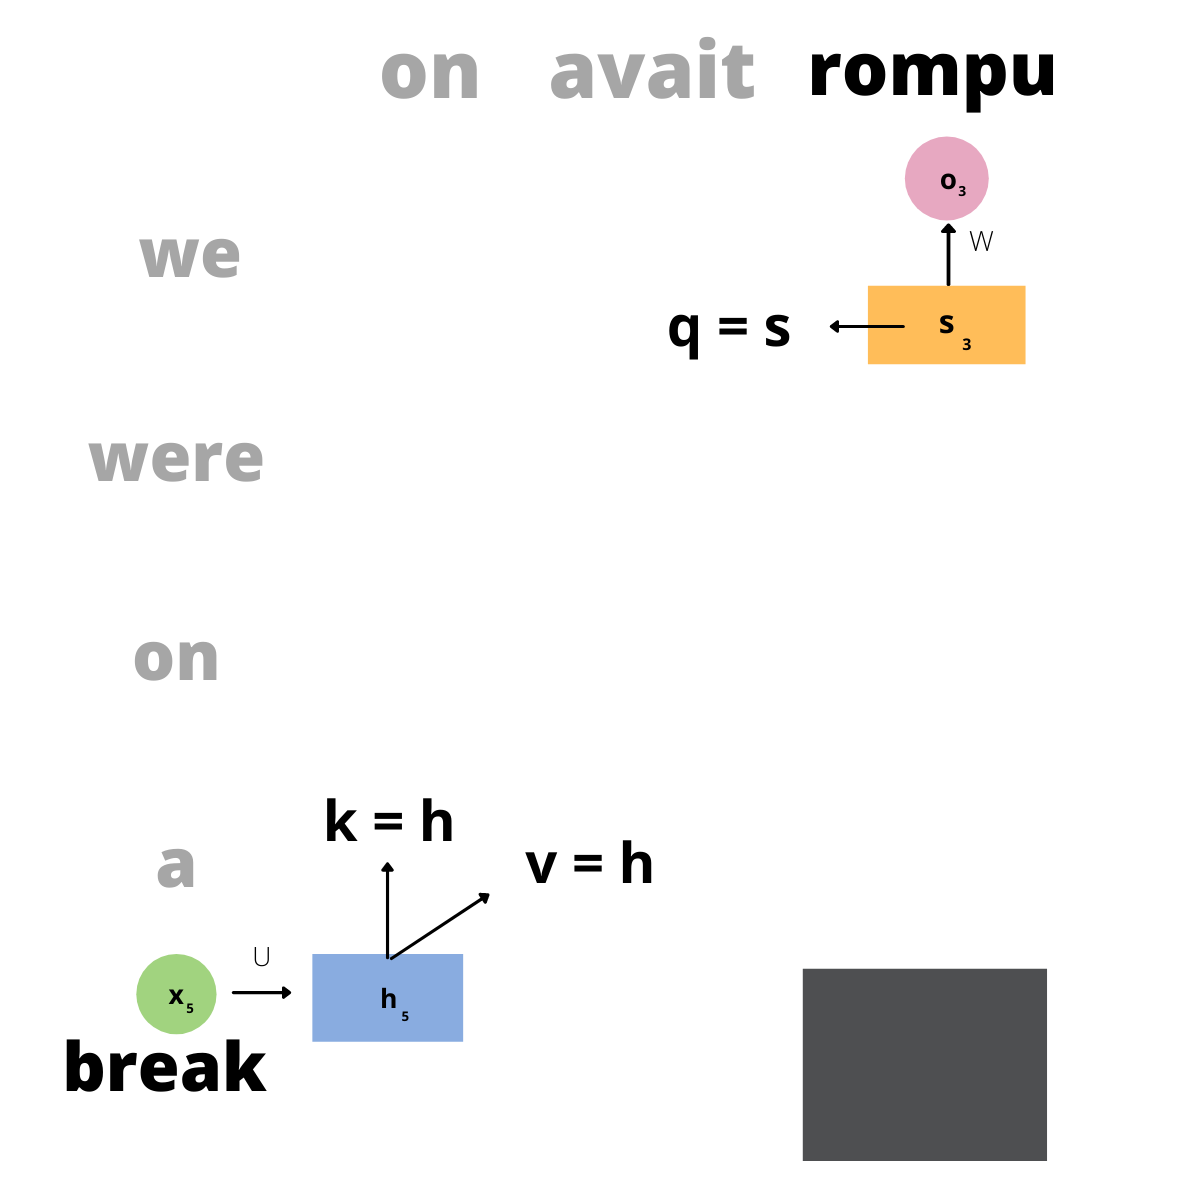
\includegraphics[width = 6cm]{images/attn_structure2.png}
\end{textblock}}
\only <4>{
\begin{textblock}{0.5}(0.55, 0.15)
        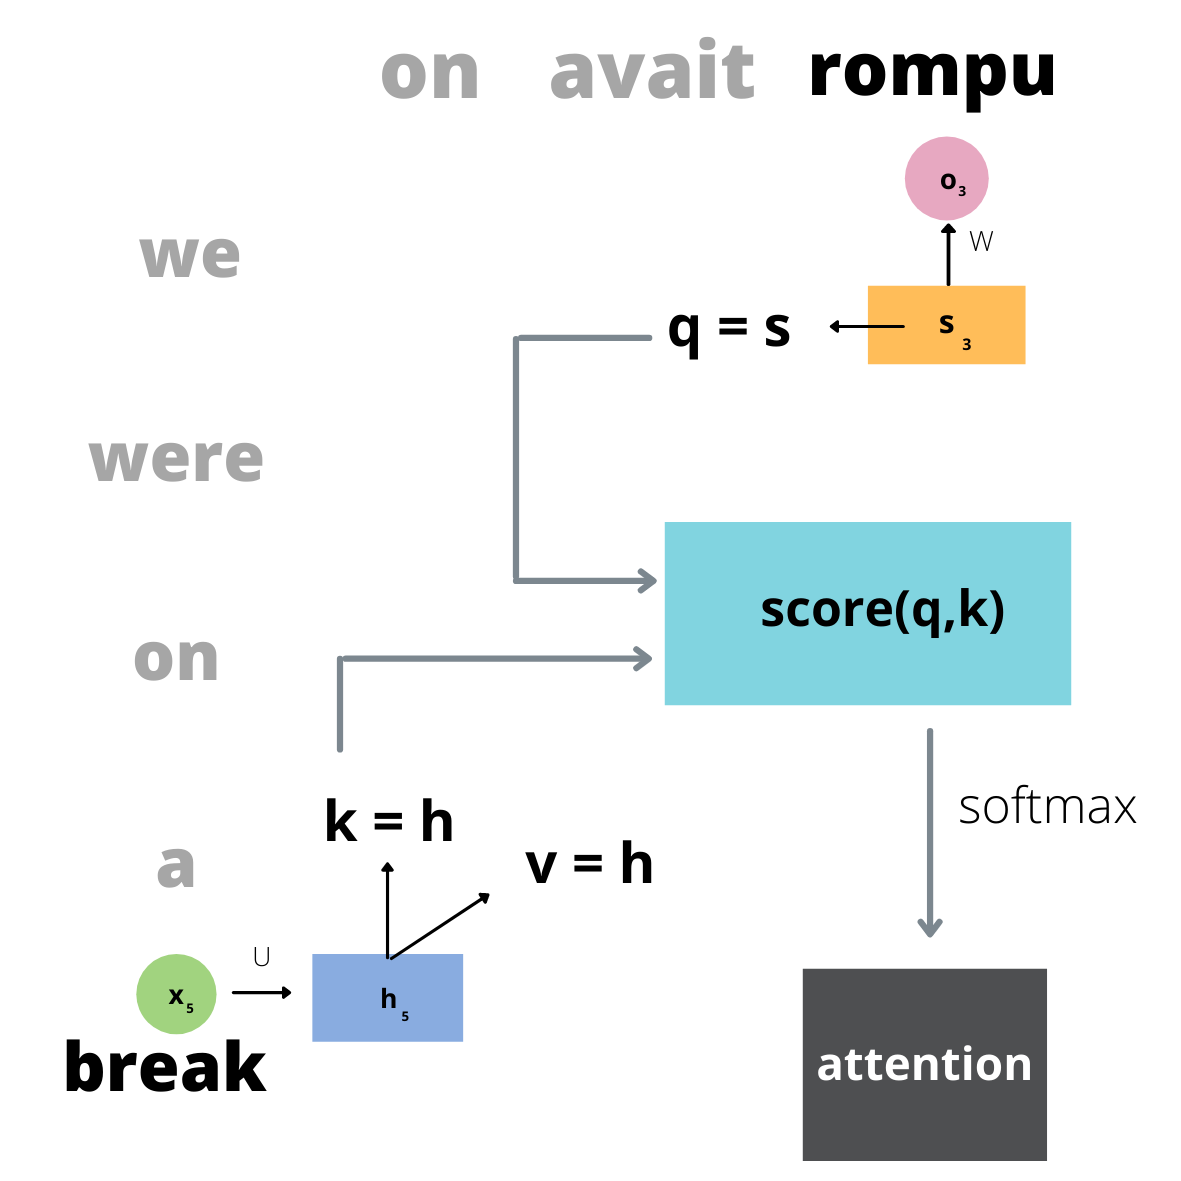
\includegraphics[width = 6cm]{images/attn_structure3.png}
\end{textblock}}
\only <5>{
\begin{textblock}{0.5}(0.55, 0.15)
        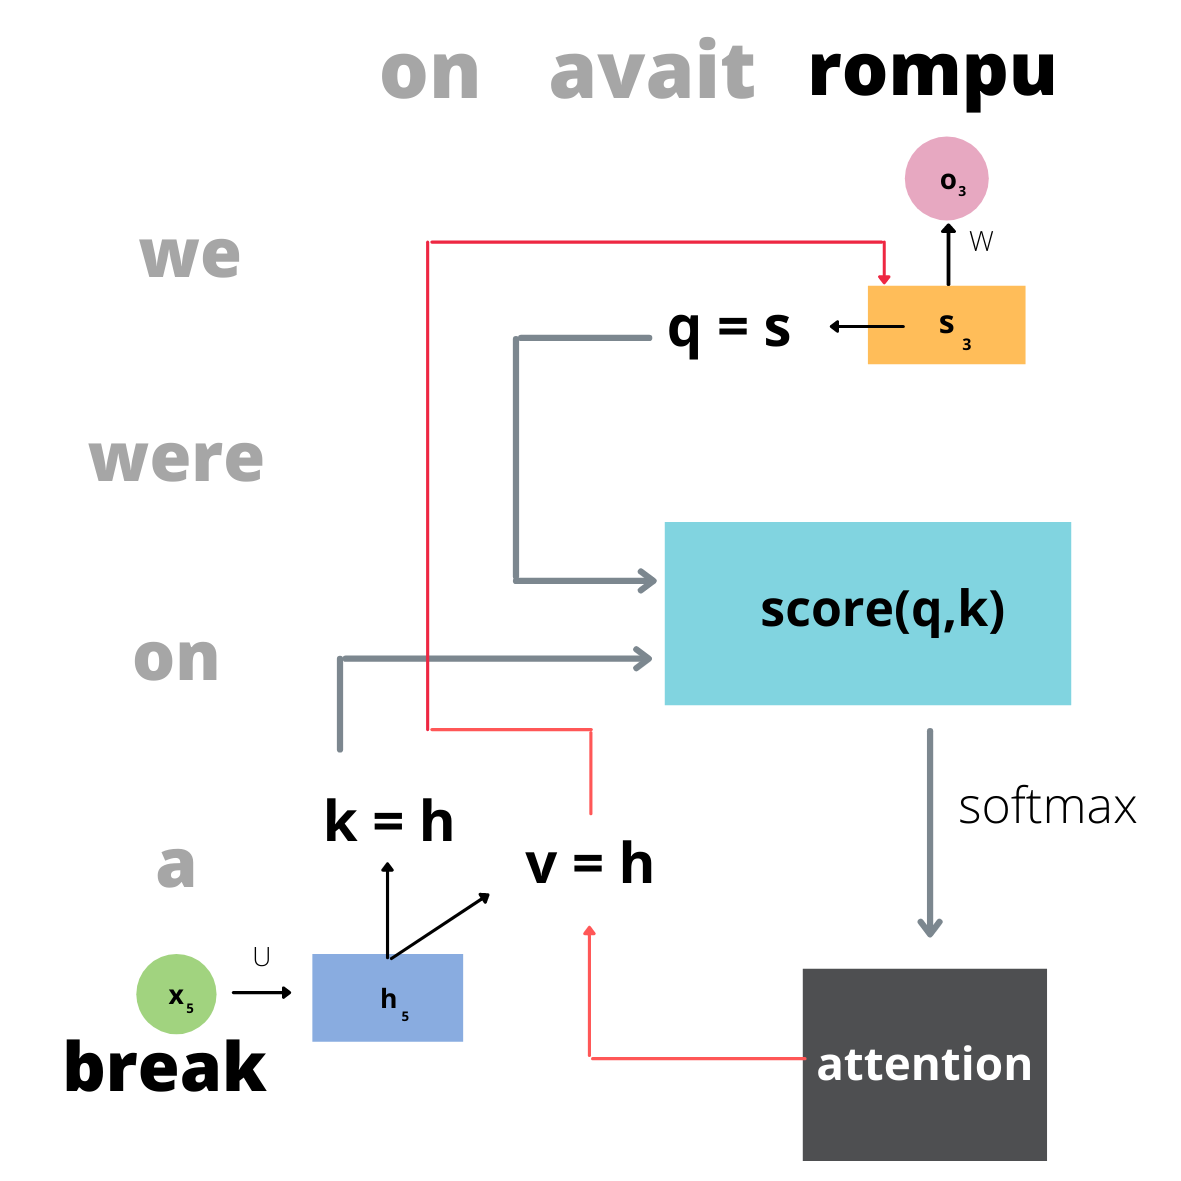
\includegraphics[width = 6cm]{images/attn_structure4.png}
\end{textblock}}
\only <6>{
\begin{textblock}{0.5}(0.5, 0.15)
        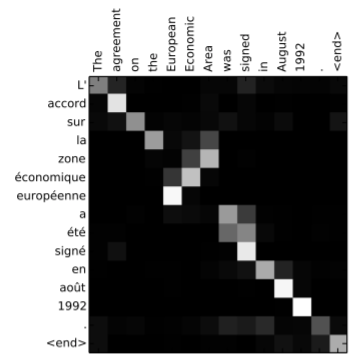
\includegraphics[width = 6cm]{images/att2.png}
\end{textblock}}
\end{frame}

\section{Transformers}
\begin{frame}
    \frametitle{Table of contents}
    \tableofcontents[currentsection]
\end{frame}
\subsection{Structure}
\begin{frame}{The Transformer}
\begin{columns}[onlytextwidth]
    \begin{column}{0.50\textwidth}
    Transformers are a novel architecture that \textbf{gets rid of any recurrency}, thus relying solely on \textbf{attention modules} \cite{transformer}. They have the following advantages:
    \begin{itemize}
        \item They allow for \textbf{parallelisation}.
        \item They are \textbf{flexible}, thus allowing its use on a wide variety of tasks. They only need to be pre-trained once and then they can be fine-tuned on specific tasks.
    \end{itemize}
    \end{column}
\end{columns}
\begin{textblock}{0.5}(0.51, 0.05)
        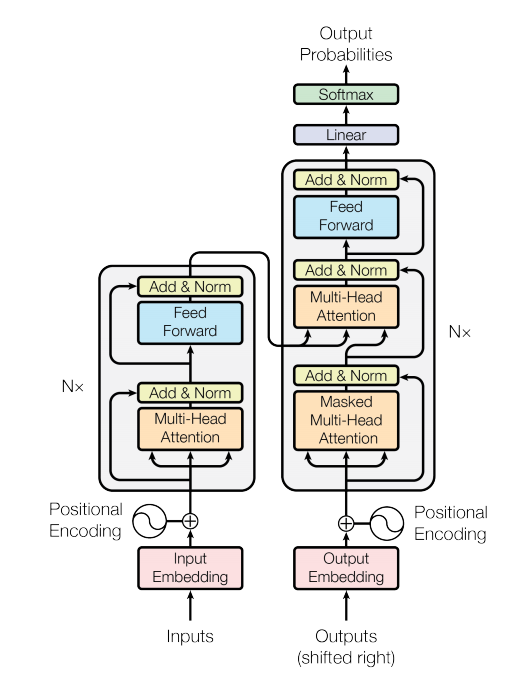
\includegraphics[width = \textwidth]{images/transformer.png}
\end{textblock}
\end{frame}
\begin{frame}{Attention in Transformers}
\begin{textblock}{0.05}(0.05, 0.19)
    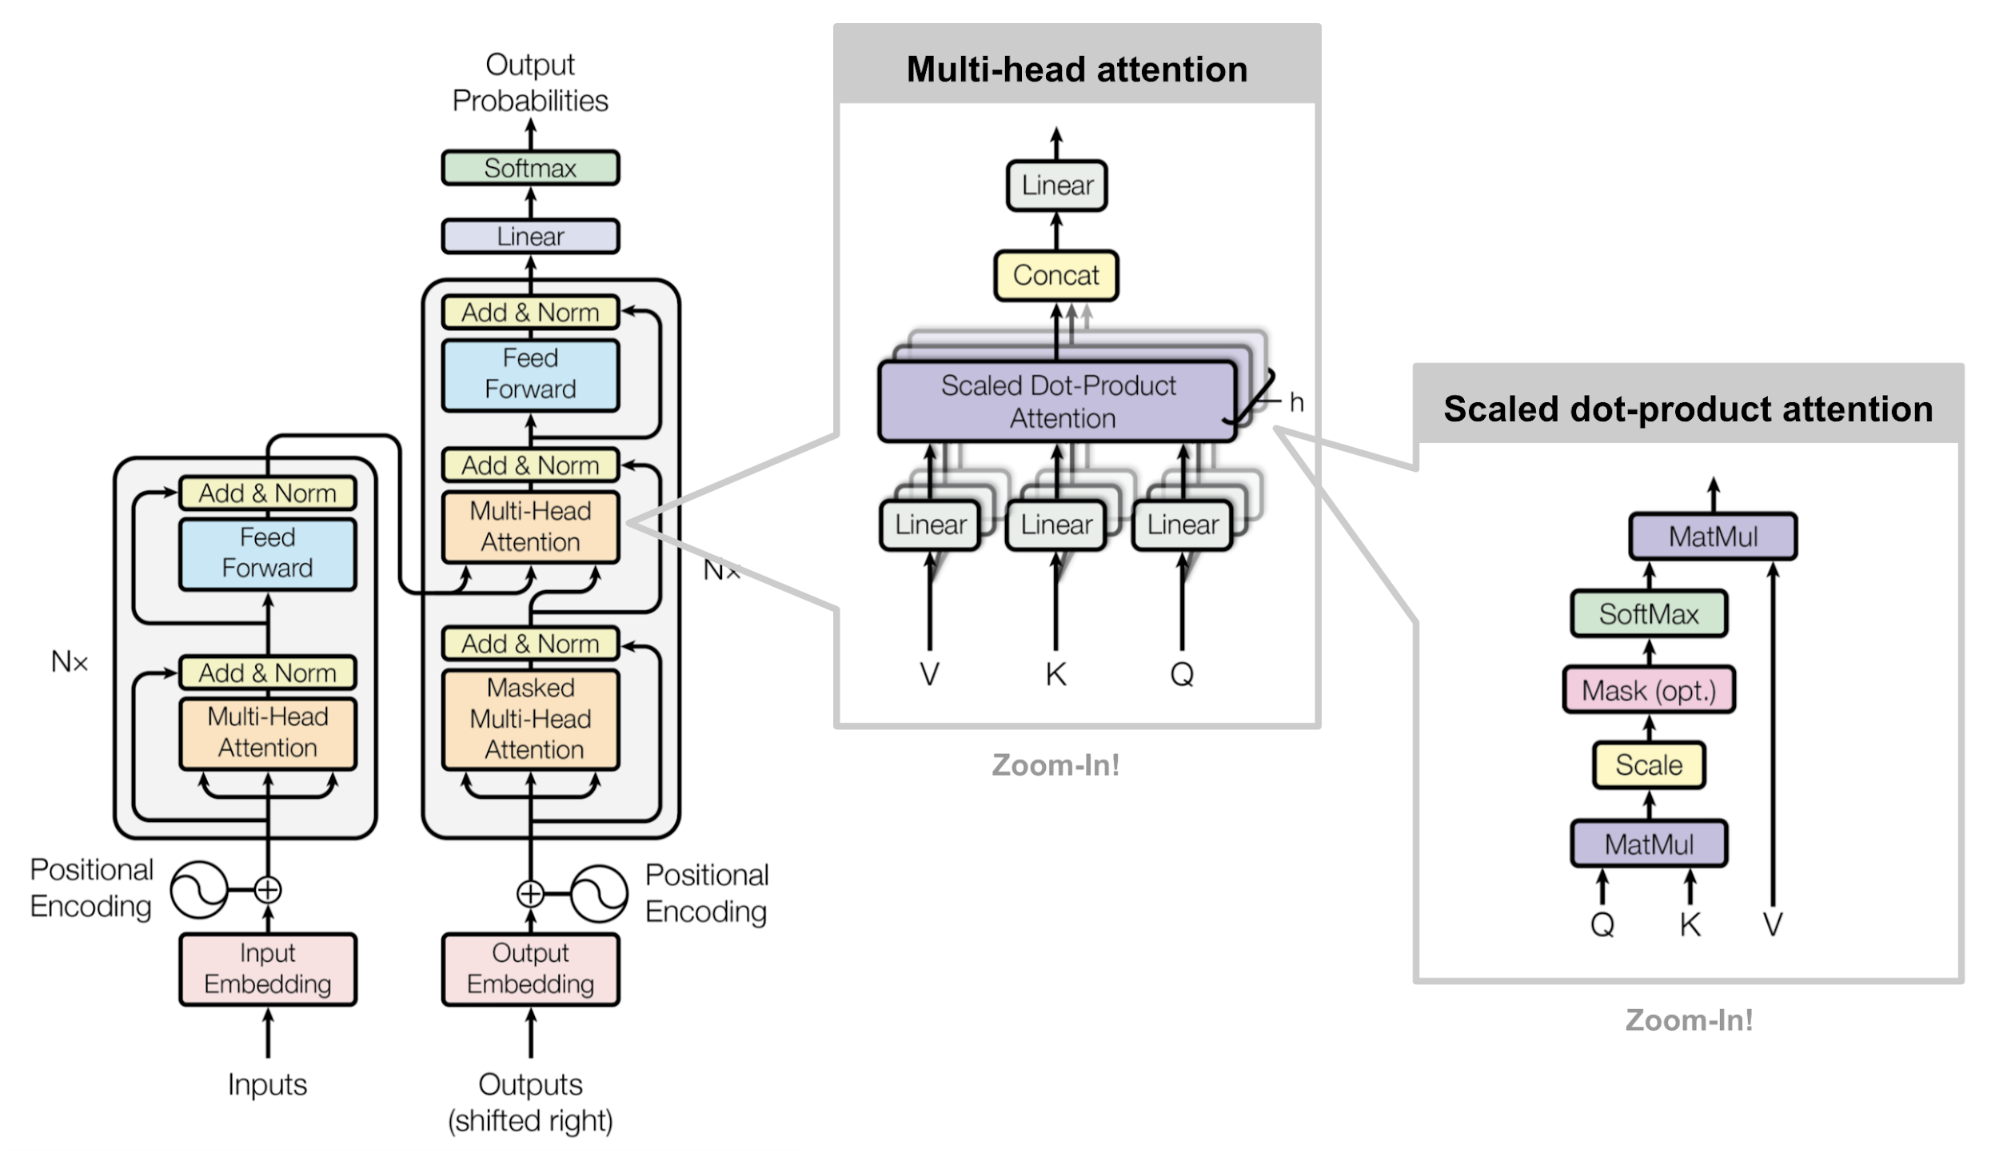
\includegraphics[width = 11.1cm]{images/att.png}
\end{textblock}
\footnote{\url{https://lilianweng.github.io/lil-log/2018/06/24/attention-attention.html#a-family-of-attention-mechanisms}}
\end{frame}
\begin{frame}{Attention in Transformers}
\begin{columns}[onlytextwidth]
    \begin{column}{0.50\textwidth}
    Their novelty in terms of attention architecture is:\\
    The use of \textbf{scaled dot-product} score function:
    \vspace{0.15cm}
    $$score(q,K_i) = \displaystyle \frac{q^TK_i}{\sqrt{d_k}} $$ \\
    The use of \textbf{multi-head attention}, that is, $h$ attention layers running in parallel.\vspace{0.15cm}\\
    $Q$, $K$ and $V$ are computed from input/output using \textbf{weight matrices} $W_q, W_K$ and $W_V$.
    \end{column}
\end{columns}
\only <1>{
\begin{textblock}{0.5}(0.51, 0.19)
        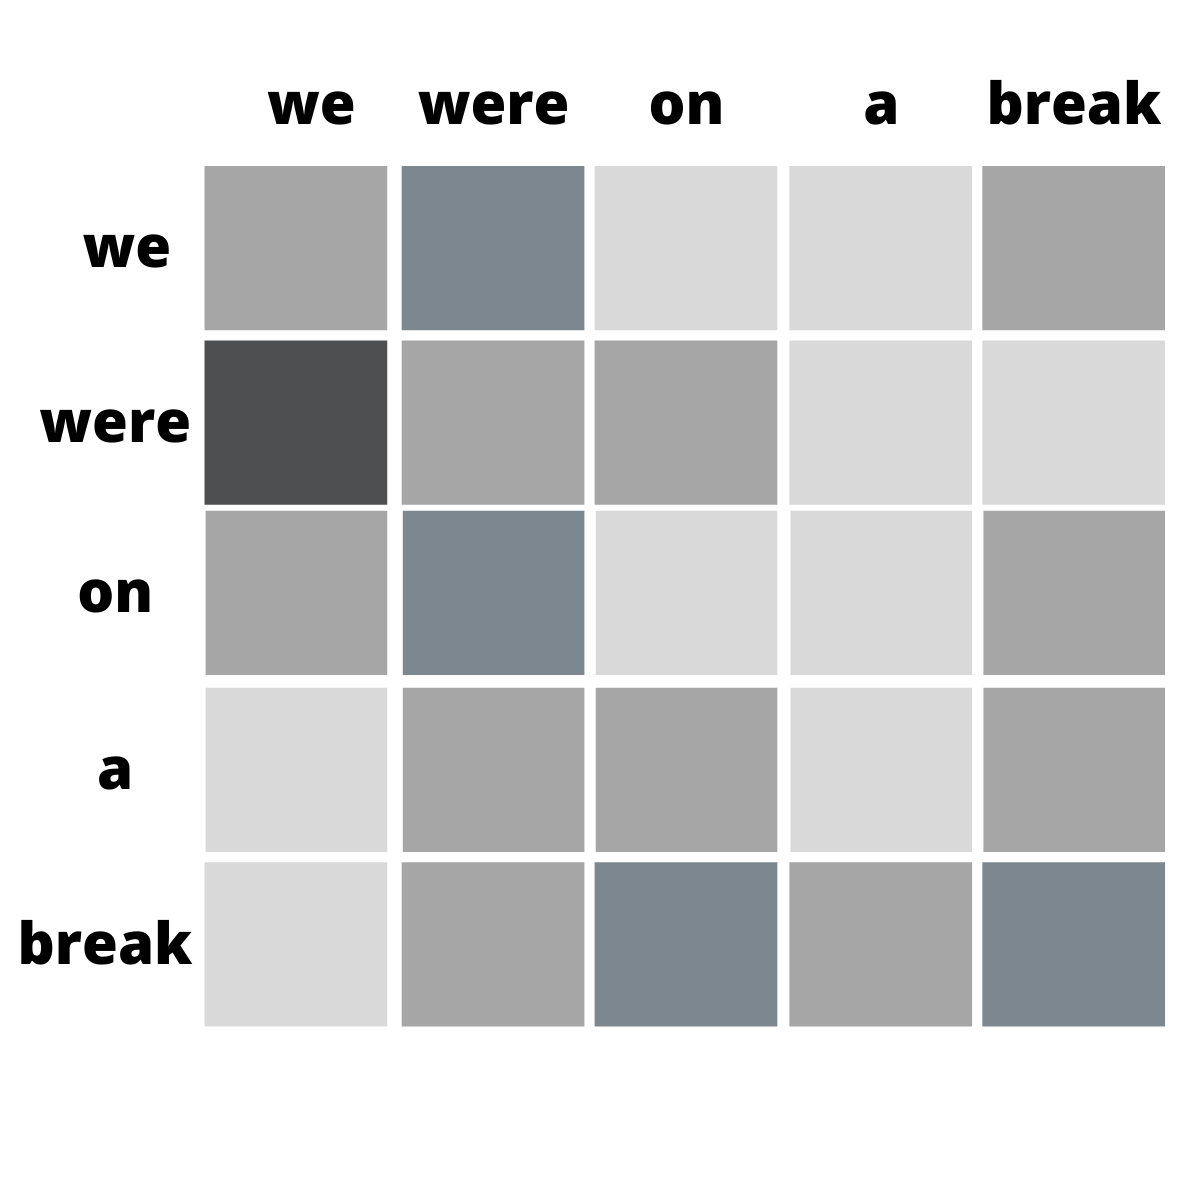
\includegraphics[width = 6cm]{images/self_attn1.png}
\end{textblock}}
\only <2>{
\begin{textblock}{0.5}(0.51, 0.19)
        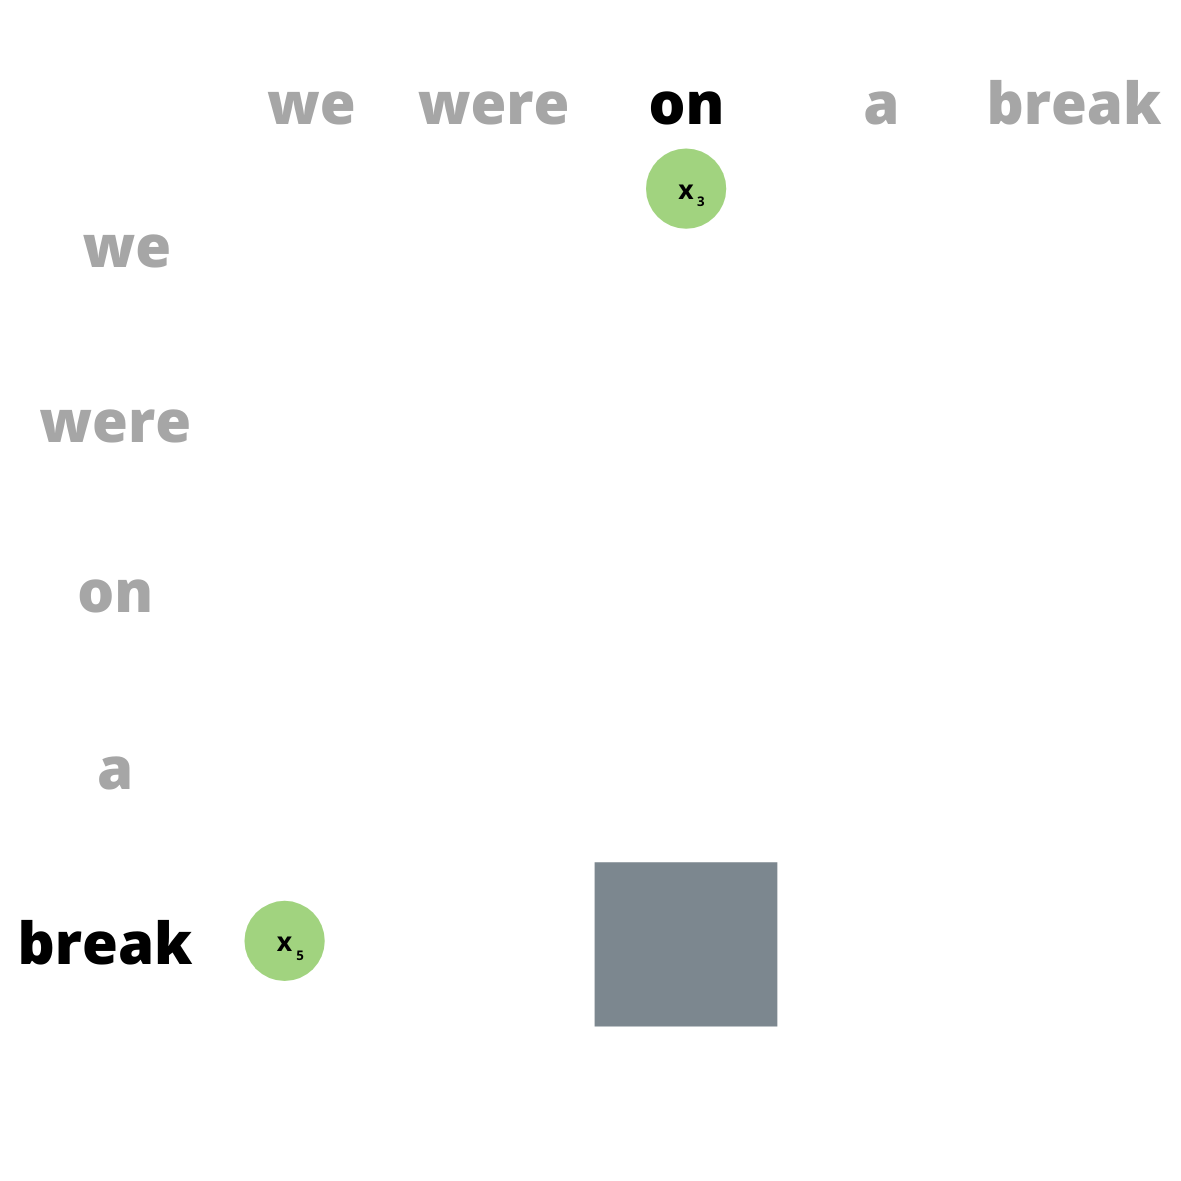
\includegraphics[width = 6cm]{images/self_attn2.png}
\end{textblock}}
\only <3>{
\begin{textblock}{0.5}(0.51, 0.19)
        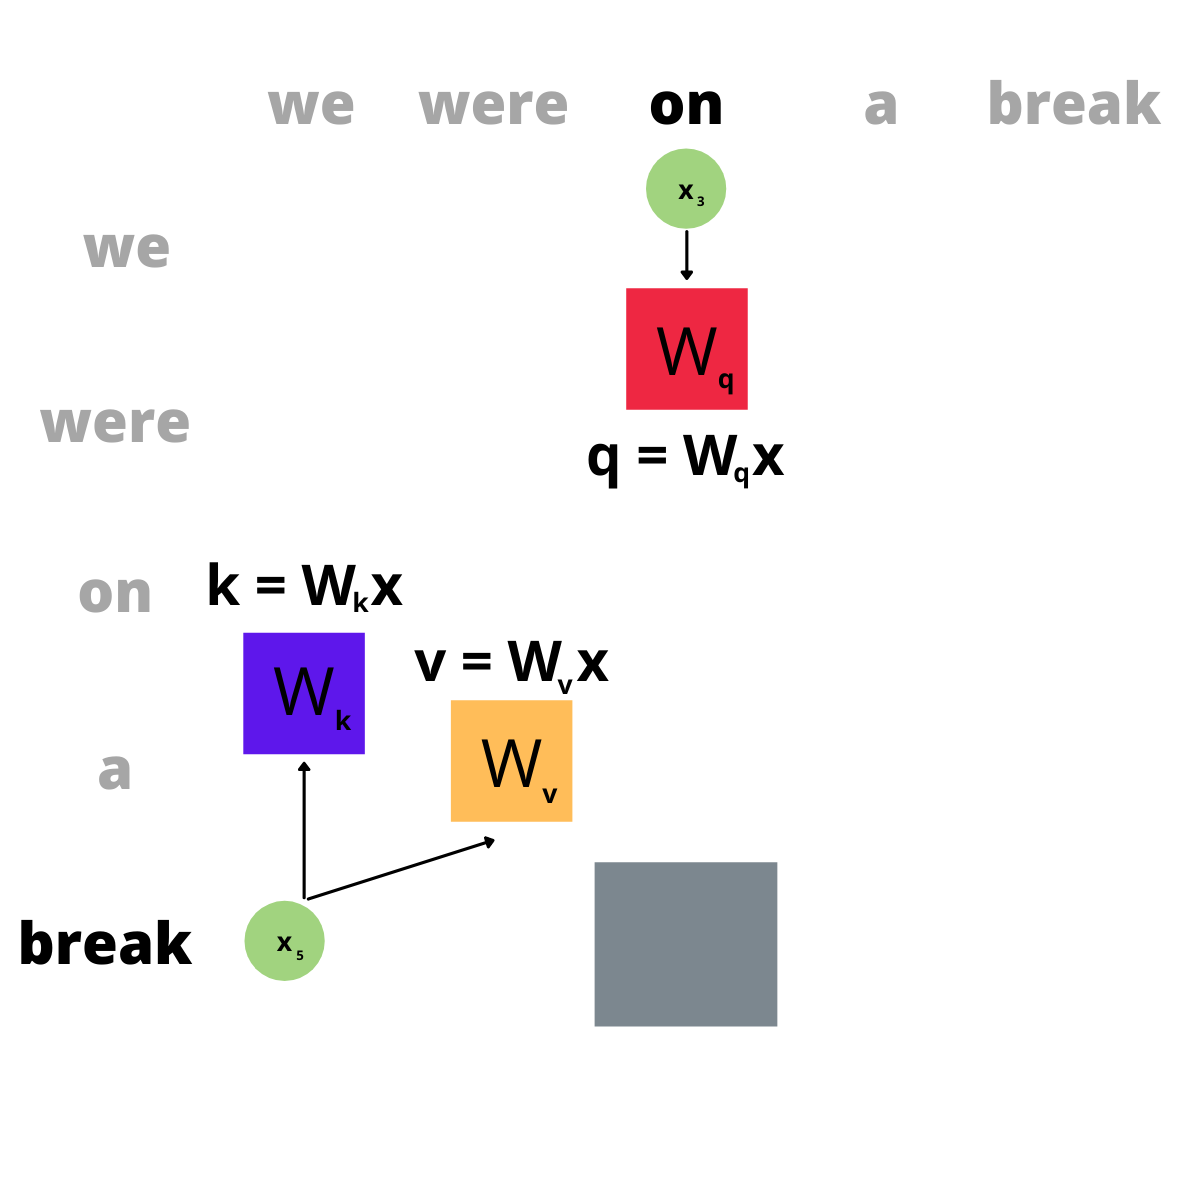
\includegraphics[width = 6cm]{images/self_attn3.png}
\end{textblock}}
\only <4>{
\begin{textblock}{0.5}(0.51, 0.19)
        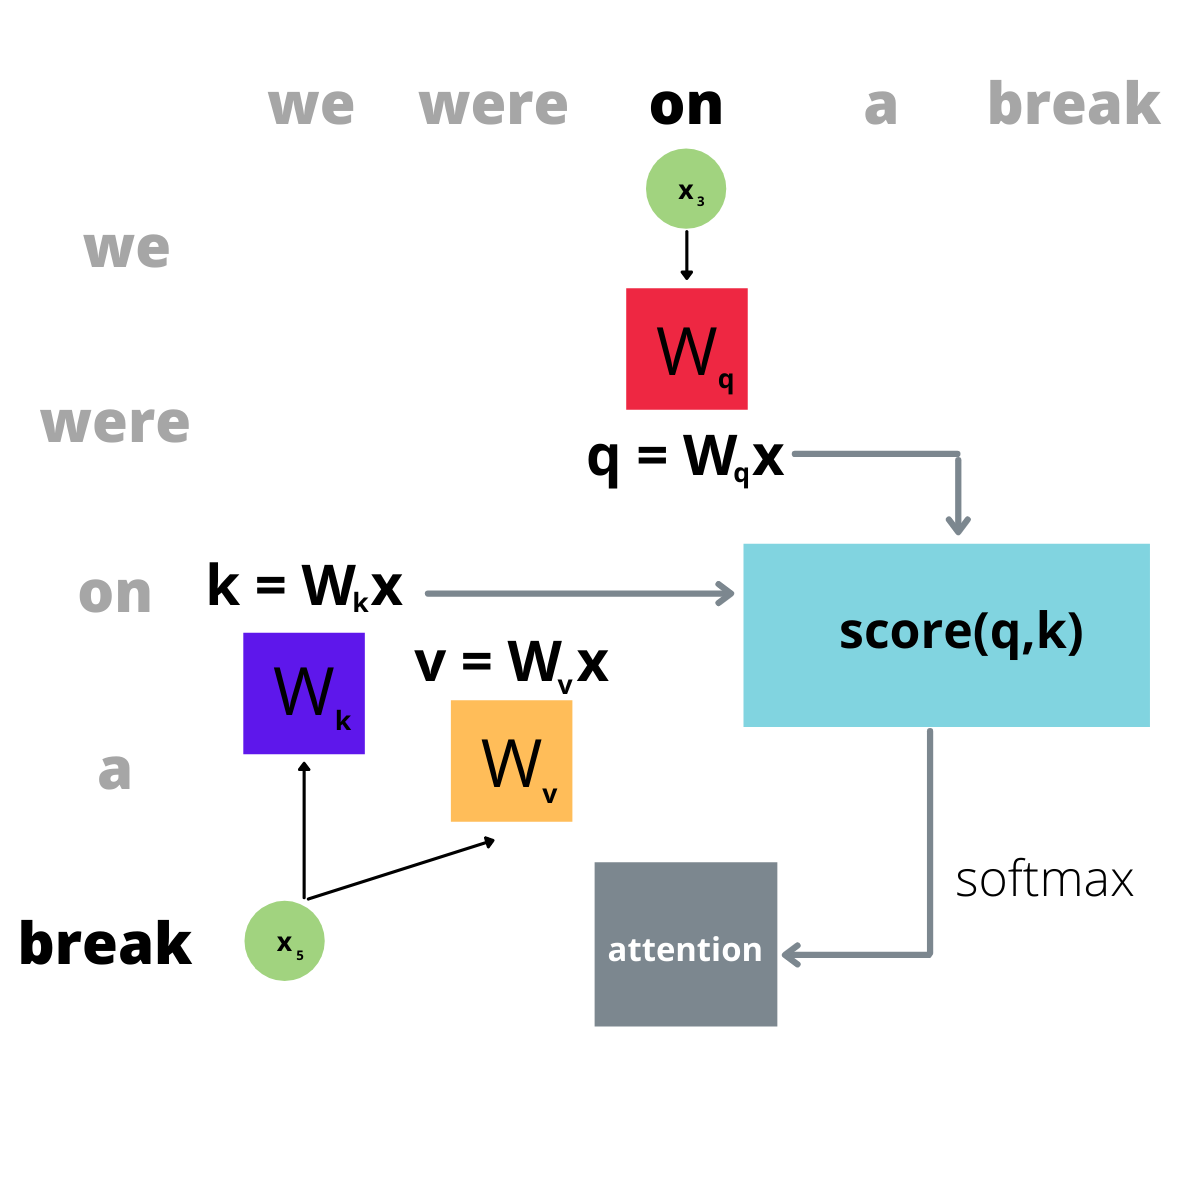
\includegraphics[width = 6cm]{images/self_attn4.png}
\end{textblock}}
\only <5>{
\begin{textblock}{0.5}(0.51, 0.19)
        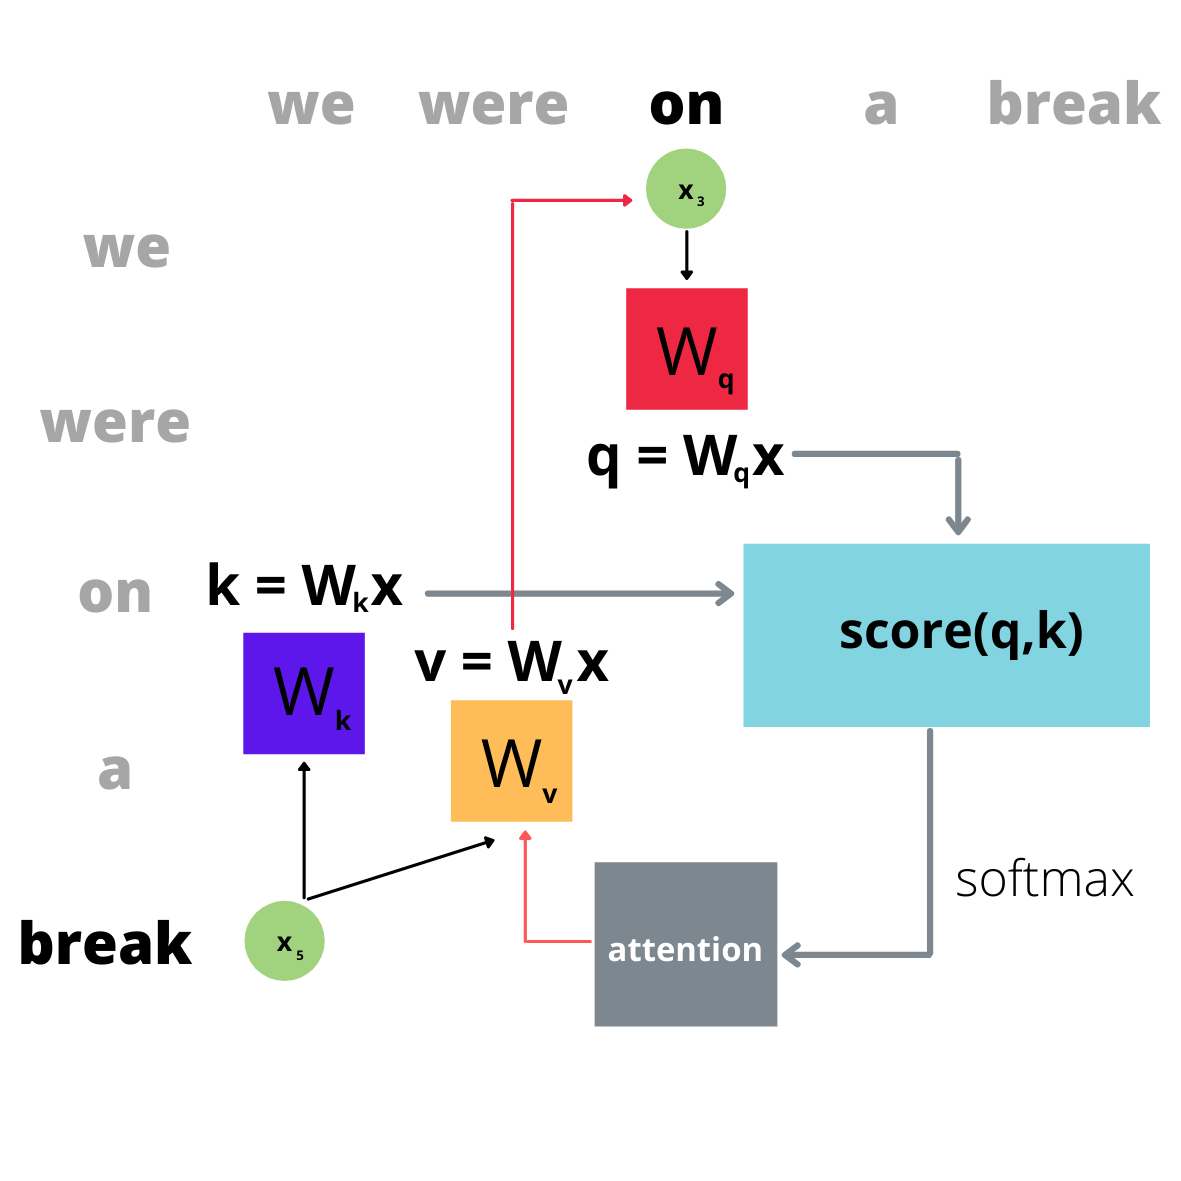
\includegraphics[width = 6cm]{images/self_attn5.png}
\end{textblock}}
\end{frame}
\subsection{BERT}
\begin{frame}{BERT: a Transformer based LM}
\begin{columns}
    \begin{column}{0.45\textwidth}
    \textbf{(BERT)}: A pre-trained Transformer based architecture that achieved state-of-the-art in several tasks, including question answering, text classification and natural language understanding \cite{bert}\footnote{Visualising attention: \url{https://huggingface.co/exbert/}}.
\vspace{0.3cm}\\ Its pre-training relies on a joint \textbf{masked LM} (15\% of tokens) and \textbf{next sentence prediction} for its pre-training process\footnote{Visualisation from: \url{http://jalammar.github.io/illustrated-bert/}}.
    \end{column}
\end{columns}
\begin{textblock}{0.5}(0.52, 0.2)
        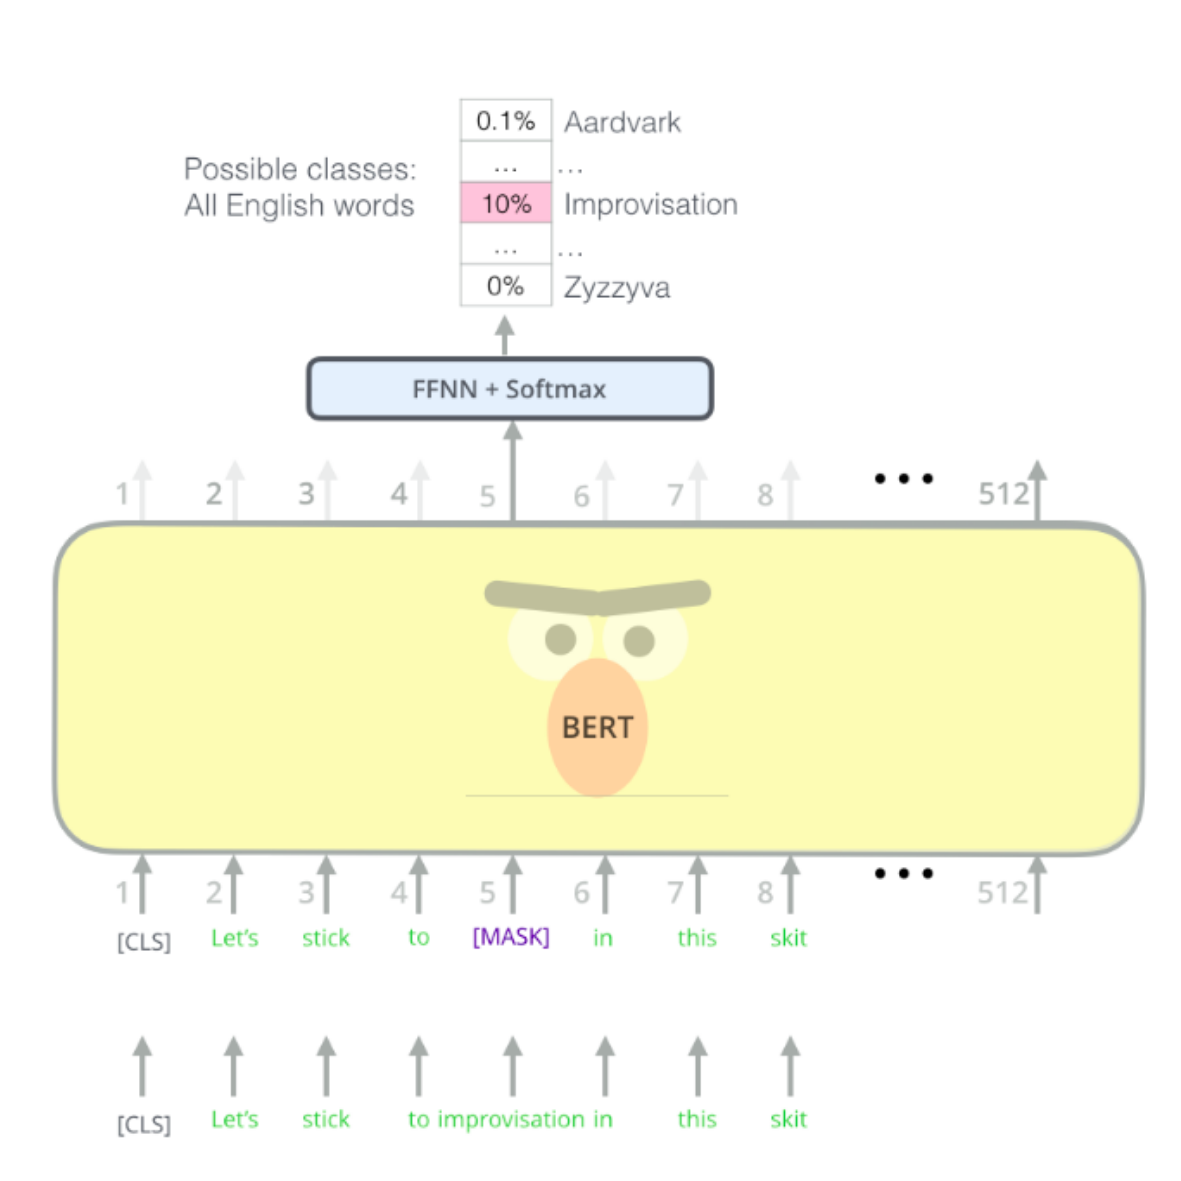
\includegraphics[width = 5.5cm]{images/bert_MLM.png}
\end{textblock}
\end{frame}
\subsection{Ethical Concerns}
\begin{frame}{Ethical Concerns with LMs}
Huge language models can be extremely dangerous \cite{parrot}:\\ They come at a \textbf{strong environmental cost}. \\
\\ They are usually trained on data that is \textbf{biased}, encoding \textbf{racism} and \textbf{sexism} in them.\\
It's \textbf{hard to track} and interpret due to their size.
\begin{columns}[onlytextwidth]
    \begin{column}{0.60\textwidth}
    \vspace{0.1cm}\\
    It is important to use this technology \textbf{carefully}, always assessing the possible negative outcomes. 
    \\Bigger is not always better!
    \end{column}
\end{columns}
\begin{textblock}{0.5}(0.65, 0.5)
        
\includegraphics[width = 3.2cm]{images/warning.png}
\end{textblock}
\end{frame}
\begin{frame}{In a Nutshell}
    \begin{itemize}
        \item \textbf{Language models} are used as a departing point for many NLP applications.
        \item They are trained with variations of \textbf{word prediction} and consuming a lot of data.
        \item \textbf{RNNs} exploit the sequential nature of data by being applied in order to each input word.
        \item \textbf{Attention} improve RNNs by allowing the model to encode complex semantics
        \item And they are used in \textbf{Transformers} for building faster and larger models.
        \item Nevertheless, we need to be careful when we use these models since they can be \textbf{harmful} for certain demographic groups and the environment.
    \end{itemize}
\end{frame}

\section{Practical Work}
\begin{frame}
    \frametitle{Table of contents}
    \tableofcontents[currentsection]
\end{frame}
\subsection{Sentiment Analysis with Transformers}
\begin{frame}{Transformer LMs for Sentiment Analysis}
    \textbf{Objective}: Students will get familiarised with the use of pre-trained models, how to interpret them and implement them in a simple NLP pipeline. \\
    \textbf{Tasks}: Building a simple sentiment classifier using a pre-trained model from HuggingFace \footnote{\url{https://huggingface.co/distilbert-base-uncased-finetuned-sst-2-english/tree/main}}. \\
    Visualising the attention weights for model understanding.\\
\begin{textblock}{0.15}(0.07, 0.55)
        
\includegraphics[width = 11cm]{images/task.png}
\end{textblock}
\end{frame}

%------------------------------------------------
\section{References}
\begin{frame}[allowframebreaks]
    \frametitle{References}
    \tiny
    \begin{thebibliography}{}
        \setbeamertemplate{bibliography item}[text]
        
        \bibitem{bengio}
        Bengio, Y., Ducharme, R., Vincent, P., & Jauvin, C. (2003). A Neural Probabilistic Language Model. The Journal of Machine Learning Research, 19.
        
        \bibitem{rnn}
        Elman, J. L. (1990). Finding structure in time. Cognitive science, 14(2), 179-211.
        
        \bibitem{lstm}
        Hochreiter, S., & Schmidhuber, J. (1997). Long Short-term Memory. Neural Computation, 9, 1735–1780. \url{https://doi.org/10.1162/neco.1997.9.8.1735}
        
        \bibitem{attention}
        Bahdanau, D., Cho, K., & Bengio, Y. (2016). Neural Machine Translation by Jointly Learning to Align and Translate. ArXiv:1409.0473 [Cs, Stat]. \url{http://arxiv.org/abs/1409.0473}
        
        \bibitem{transformer}
        Vaswani, A., Shazeer, N., Parmar, N., Uszkoreit, J., Jones, L., Gomez, A. N., Kaiser, Ł., & Polosukhin, I. (2017). Attention is All you Need. Advances in Neural Information Processing Systems, 30, 5998–6008. \url{https://arxiv.org/abs/1706.03762}
        
        \bibitem{bert}
        Devlin, J., Chang, M.-W., Lee, K., & Toutanova, K. (2019). BERT: Pre-training of Deep Bidirectional Transformers for Language Understanding. Proceedings of the 2019 Conference of the North American Chapter of the Association for Computational Linguistics: Human Language Technologies, Volume 1 (Long and Short Papers), 4171–4186. \url{https://doi.org/10.18653/v1/N19-1423}
        
        \bibitem{parrot}
        Bender, E. M., Gebru, T., McMillan-Major, A., & Shmitchell, S. (2021). On the Dangers of Stochastic Parrots: Can Language Models Be Too Big? Proceedings of the 2021 ACM Conference on Fairness, Accountability, and Transparency, 610–623. \url{http://faculty.washington.edu/ebender/papers/Stochastic_Parrots.pdf}

    \end{thebibliography}
\end{frame}

\end{document}